%% Future Generation Computer Systems -- Full Length Article (elsarticle, two-column).
\documentclass[5p,twocolumn]{elsarticle}

\usepackage{amsmath}
\usepackage{newtxtext,newtxmath}
\usepackage{graphicx}
\usepackage{booktabs,array}
\usepackage{seqsplit}
\usepackage[hidelinks]{hyperref}
\biboptions{sort&compress}
\renewcommand{\dbltopfraction}{0.95}
\renewcommand{\topfraction}{0.95}
\renewcommand{\textfraction}{0.05}
\renewcommand{\dblfloatpagefraction}{0.6}
\renewcommand{\floatpagefraction}{0.6}
\setcounter{dbltopnumber}{3}
% Generated by manuscript/fgcs/tools/a3_numbers.py from analysis_a3.json (SHA-256 33e11a858ea338b3c3ff25bec2f59527a3a2100a386658443def77956501cee0).
% Do not edit by hand.
\newcommand{\AiiiRetainedOne}{8}
\newcommand{\AiiiCostOne}{0}
\newcommand{\AiiiRefCostOne}{22}
\newcommand{\AiiiCellsOne}{24}
\newcommand{\AiiiVerdictOne}{rarely consolidates}
\newcommand{\AiiiRetainedZeroOne}{4}
\newcommand{\AiiiRetainedTwoPctOne}{14}
\newcommand{\AiiiCostAllOne}{0}
\newcommand{\AiiiRetainedTwo}{20}
\newcommand{\AiiiCostTwo}{0}
\newcommand{\AiiiRefCostTwo}{13}
\newcommand{\AiiiCellsTwo}{32}
\newcommand{\AiiiVerdictTwo}{rarely consolidates}
\newcommand{\AiiiRetainedZeroTwo}{7}
\newcommand{\AiiiRetainedTwoPctTwo}{29}
\newcommand{\AiiiCostAllTwo}{0}
\newcommand{\AiiiUnitsOne}{2{,}730}
\newcommand{\AiiiUnitsTwo}{1{,}200}
\newcommand{\AiiiDetects}{12}
\newcommand{\AiiiFrames}{14}
\newcommand{\AiiiRhoMin}{0.30}
\newcommand{\AiiiRhoMax}{0.66}
\newcommand{\AiiiNotDetected}{tier-1 TimeTrack and tier-2 LSTM fastStorage}
\newcommand{\AiiiValWorseMin}{84}
\newcommand{\AiiiValWorseMax}{98}
\newcommand{\AiiiOutWorseMin}{66}
\newcommand{\AiiiOutWorseMax}{94}
\newcommand{\AiiiBAMin}{0.48}
\newcommand{\AiiiBAMax}{0.65}
\newcommand{\AiiiGroupModels}{2.4}
\newcommand{\AiiiShareModelsLSTM}{3.7}
\newcommand{\AiiiGroupRetained}{53}
\newcommand{\AiiiGroupParams}{124{,}180}
\newcommand{\AiiiSTwoParams}{206{,}100}
\newcommand{\AiiiMOneParams}{52{,}500}
\newcommand{\AiiiGroupParamCut}{40}
\newcommand{\AiiiGroupCost}{0}
\newcommand{\AiiiGroupVerdict}{grouping adds savings}
\newcommand{\AiiiGroupMaxRatio}{1.004}
\newcommand{\AiiiMOneMaxRatio}{1.057}
\newcommand{\AiiiMOneCostLSTM}{6}
\newcommand{\AiiiGroupMacroBelow}{3}
\newcommand{\AiiiMOneMacroBelow}{5}
\newcommand{\AiiiGroupWorstGain}{-5.74}
\newcommand{\AiiiMOneWorstGain}{-24.56}
\newcommand{\AiiiGroupWinMin}{26}
\newcommand{\AiiiGroupWinMax}{53}
\newcommand{\AiiiGroupTwoPctModels}{2.1}
\newcommand{\AiiiGroupTwoPctCost}{1}
\newcommand{\AiiiOracleModels}{2.8}
\newcommand{\AiiiOracleMinRatio}{0.986}
\newcommand{\AiiiFixedNoCost}{2}
\newcommand{\AiiiFixedShared}{14}
\newcommand{\AiiiFallbackPositive}{3}
\newcommand{\AiiiFallbackCells}{16}
\newcommand{\AiiiFallbackBefore}{0}



\journal{Future Generation Computer Systems}

\begin{document}

\begin{frontmatter}

\title{Contextual Input versus Representation Sharing in Multi-Metric Runtime Forecasting: Selective Gains and a Recurring Sharing Cost}

\author[uva]{Abdelhak Kadouma\corref{cor1}}
\ead{abdelhak.kadouma@uwasa.fi}
\author[uva,sau]{Amit K. Shukla}
\ead{amit.shukla@uwasa.fi}
\ead{amitkshukla@sau.int}
\author[uva]{Mohammed Elmusrati}
\ead{moel@uwasa.fi}

\cortext[cor1]{Corresponding author}

\affiliation[uva]{organization={University of Vaasa},
  city={Vaasa},
  country={Finland}}
\affiliation[sau]{organization={Department of Computer Science and Engineering, South Asian University},
  addressline={Gaushala Rd., Maidan Garhi},
  city={New Delhi},
  postcode={110068},
  country={India}}

\begin{abstract}
Cloud telemetry forecasting involves two separate choices:
whether a target's model receives other resources' histories (contextual
input) and whether several resource targets share one model (representation
sharing). Channel-independent versus channel-dependent comparisons change
both at once. A $2\times2$ design of independent or shared models with
own-resource or all-resource input separates them for central processing unit
(CPU), throughput, memory and disk-write forecasting: with long short-term
memory (LSTM) networks on two Bitbrains environments and three dependent
Materna blocks, with TimeTrack as development data, and with LSTM, DLinear,
PatchTST-style and iTransformer-style backbones on 20 Bitbrains virtual
machines. Protocols were frozen before execution, and effects were checked
with sensitivity controls, machine-level bootstrap intervals and persistence
skill. Sharing carried a recurring cost: for a typical machine the shared
model was less accurate in all 24 LSTM comparisons and in 30 of 32 backbone
cells (13 by over 1\%, 6 of 8 for the LSTM). Contextual input helped
selectively: on the 20 VMs, typical-cell ratios against own-input models
stayed between 0.981 and 1.035, and no context effect held for every backbone. The cost is
visible before deployment: the shared model validated worse in
\AiiiValWorseMin--\AiiiValWorseMax\% of units, so a
gate sharing only within 1\% consolidated \AiiiRetainedOne--\AiiiRetainedTwo\%
of units, whereas validation-chosen grouping kept about half of the LSTM's
model reduction at a typical-cell cost below 0.5\%, though some aggregate costs
remained.
Shared-LSTM task gradients were near orthogonal but unequal in magnitude;
loss balancing narrowed the cost only slightly. No backbone beat persistence
for CPU or throughput.
\end{abstract}

\begin{keyword}
runtime forecasting \sep cloud telemetry \sep multi-metric forecasting \sep multi-task learning \sep contextual input \sep representation sharing \sep negative transfer diagnostics
\end{keyword}

\end{frontmatter}


\section{Introduction}
\label{sec:introduction}

Engineers who forecast cloud runtime telemetry for resource management
\citep{Taherizadeh2018Monitoring,Bauer2020SelfAware} decide two things:
whether a target's forecaster should receive other resources' telemetry, and
whether several targets should share one model. Comparisons of
channel-independent and channel-dependent forecasters
\citep{Han2024ChannelIndependent} change both at once, because a
channel-independent model shares one set of weights across channels that it
processes separately, whereas a channel-dependent model mixes channels inside
one shared model; which decision costs accuracy therefore remains unknown.
Separating them, we find that sharing, not contextual input, carries the
recurring cost: for a typical machine the shared model was less accurate in
all 24 LSTM block--resource comparisons, on Bitbrains, Materna and the
TimeTrack development data, and in 30 of 32 cells of four backbones, whereas
context effects were small and model-dependent. The cost is already visible in ordinary inner
validation, so validation can guide which resources to share.

Runtime-series benchmarking spans statistical, neural and foundation models
\citep{DiMenna2026RuntimeForecasting}, and cloud studies combine multivariate
resource inputs with joint multi-output prediction
\citep{Ullah2023CloudBiLSTM,Tripathi2025MMRP}. Multi-task learning offers
inductive transfer between related tasks \citep{Caruana1997Multitask}, but
which tasks to share, and how, must be evaluated
\citep{Standley2020TaskGrouping,Fifty2021TaskGroupings,Nochumsohn2025MTLinear},
and two practical questions are rarely tested for telemetry: whether the
validation data available before deployment show when sharing will cost
accuracy, and whether sharing only some resources keeps the savings without
the cost.

We separate the two decisions with a $2\times2$ design
(Figure~\ref{fig:sharing-framework}). Independent target models receive
own-resource histories (S1) or all-resource histories (S2); one shared model
with resource-specific outputs receives own-resource histories (M0) or
all-resource histories (M1). Context is then varied with sharing held fixed
(S2:S1, M1:M0), and sharing with input held fixed (M0:S1, M1:S2). The
independent all-input control S2 is what channel-independent versus
channel-dependent comparisons lack. The targets are CPU utilisation,
throughput, memory usage and disk-write activity.

The first part of the study (tier~1) evaluates S1, S2 and M1 with an LSTM on
the Bitbrains fastStorage and Rnd environments and three dependent Materna
blocks, with TimeTrack as development data and post-hoc controls for context
selection, capacity and model family (Section~\ref{sec:posthoc-controls}). The
second part (tier~2) adds M0 and repeats the $2\times2$ for DLinear,
PatchTST-style and iTransformer-style backbones on 20 Bitbrains VMs, with
diagnostics of dependence, gradients, loss shares and transfer
(Section~\ref{sec:tier2-design}). Amendment A1 tests loss balancing in the
shared LSTM (Section~\ref{sec:a1-design}), and A3 applies validation-gated
consolidation and task grouping to the existing fits
(Section~\ref{sec:a3-design}). Each part was frozen before its outcomes were
computed, and Section~\ref{sec:validation-strategy} maps every threat to its
mechanism. We make four contributions:

\begin{enumerate}
  \item \emph{An isolating design.} A $2\times2$ decomposition with the
    independent all-input control S2 varies contextual input and
    representation sharing one at a time on two Bitbrains environments,
    three Materna blocks and four backbone families, under leakage control,
    matched support and protocols frozen before execution.
  \item \emph{A recurring sharing cost and selective context.} The
    typical-cell cost of sharing recurs in direction in 54 of 56 cells across
    both tiers. It is clear for the LSTM, whose median-ratio interval lies
    above one in 7 of 8 tier-2 cells, and its tier-1 throughput, memory and
    disk-write penalties survive common-context and approximately
    capacity-matched controls. Context effects are selective: for the
    PatchTST-style backbone added context lowered accuracy, with intervals
    above one in 4 of 8 cells, as \citet{Han2024ChannelIndependent} lead one
    to expect.
  \item \emph{Imbalance rather than conflict.} In the shared LSTM the cost
    accompanies near-orthogonal but strongly unequal task gradients, so the
    premise of conflict-removing remedies does not hold; frozen loss balancing
    that passed its manipulation check improved the shared LSTM by at most
    0.4\% in median matched-cell error, a small part of the cost.
  \item \emph{Deciding consolidation from validation.} Under rules frozen
    before any outcome was computed, inner validation ranked machines by their
    sharing cost in \AiiiDetects{} of \AiiiFrames{} settings, a 1\% gate
    rarely consolidates, and validation-selected task grouping keeps about
    half of the LSTM's model reduction at a typical-cell cost below 0.5\%.
\end{enumerate}

\section{Related Work}
\label{sec:related-work}

Runtime telemetry supports configuration and resource-management decisions in
cloud and self-adaptive software systems
\citep{Taherizadeh2018Monitoring,Bauer2020SelfAware}, and prediction-based
provisioning and service-quality forecasting connect forecast accuracy with
software design \citep{Calheiros2015ARIMA,Syu2017DynamicQoS}. Forecast quality
nevertheless differs from controller effectiveness \citep{Qu2018Autoscaling};
the question here concerns input selection and model management, not a
measured autoscaling benefit. Multivariate covariates, hybrid resource
predictors, joint outputs and multi-provider evaluation are established
\citep{Tran2018MultivariateFuzzy,Xu2022esDNN,Tripathi2025MMRP,
Rossi2025CloudUncertainty,Zhang2025SWTCLSTM}, alongside online resource and
microservice-indicator forecasting \citep{Gao2026OMCR,Gao2026MaMiClif}.
\citet{DiMenna2026RuntimeForecasting} fit conventional models independently
per series and apply foundation models zero-shot, whereas
\citet{Ullah2023CloudBiLSTM} forecast ten channels jointly with a common
BiLSTM on fastStorage and Rnd. TimeTrack's reported resource correlations
\citep{Meliani2025TimeTrack} motivate contextual inputs but do not establish
predictive value conditional on the target's own history.

\paragraph{Channel independence and dependence} In multivariate forecasting,
the closest debate contrasts channel-independent (CI) and channel-dependent
(CD) models. \citet{Han2024ChannelIndependent} show that CD models have
higher capacity but are less robust to distribution drift, whereas CI trades
capacity for robustness. Channel clustering groups similar channels between
these extremes \citep{Chen2024ChannelClustering}, and TimeXer treats other
series as exogenous inputs to a target \citep{Wang2024TimeXer}. PatchTST
reuses embedding and Transformer weights across independently processed
channels \citep{Nie2023PatchTST}, so channel independence is shared
parameters with own-channel input, the arrangement our design calls M0; a CD
model that mixes channels in one network corresponds to M1. DLinear
forecasts trend and residual components with linear maps
\citep{Zeng2023DLinear}, and iTransformer models relationships between
variate tokens through attention \citep{Liu2024iTransformer}; tier~2
evaluates declared adaptations of all three. DeepAR and global forecasting
share functions across series rather than presenting them as simultaneous
covariates \citep{Salinas2020DeepAR,MonteroManso2021GlobalForecasting}. Our
design differs from CI-versus-CD comparisons in three ways: it adds the
independent all-input control S2 and the independent own-input S1, so that
input scope and sharing are varied one at a time; it evaluates each resource
target separately, including the consolidation it buys; and it uses cloud
telemetry with matched, leakage-controlled support. In cloud resource
forecasting, MMRP compares univariate and multivariate single-target
forecasts \citep{Tripathi2025MMRP}, an S1--S2-related precedent without a
joint resource-sharing arm, and Ullah's joint BiLSTM shares a representation
without an independent all-input target-model bridge.

\paragraph{Multi-task learning and adverse transfer} Shared learning can
provide an inductive bias \citep{Caruana1997Multitask}, but its value depends
on tasks, data and sharing structure \citep{Yu2025MultitaskFundamentals}.
Task grouping examines which tasks should learn together under accuracy and
computational constraints \citep{Standley2020TaskGrouping,Fifty2021TaskGroupings}.
Multi-objective and gradient-modification methods address conflicting updates
\citep{Sener2018MultiObjective,Yu2020GradientSurgery}, and loss-balancing
methods address unequal task-gradient magnitudes \citep{Chen2018GradNorm}.
\citet{Nikentari2022NARMAXLSTM} combine lagged station inputs with shared LSTM
layers and discuss negative transfer, MTLinear analyses gradient conflict,
balance and grouping for variate groups \citep{Nochumsohn2025MTLinear}, and
\citet{Bi2019CloudMultitask} report training-speed comparisons for cloud
multi-task forecasting. None of these establishes an independent all-input
target-model bridge or a measured target-consolidation trade-off;
Supplementary Table~S14 codes these designs against ours (Supplementary
Section~S-A). Our diagnostics measure gradient conflict, gradient magnitude,
loss shares and pairwise transfer for the LSTM
(Section~\ref{sec:tier2-analysis}). Amendment A1 then applies two
loss-balancing methods, GradNorm \citep{Chen2018GradNorm} and uncertainty
weighting \citep{Kendall2018Uncertainty}, to test the magnitude account
(Section~\ref{sec:a1-design}); gradient-modification and task-grouping
methods are not applied.

\section{Multi-Metric Runtime Forecasting Framework}
\label{sec:framework}

The framework treats two design decisions separately: which resource
histories a target's forecaster receives (\emph{contextual input}) and
whether the four targets are forecast by independent models or by one model
whose parameters they share (\emph{representation sharing}).
Figure~\ref{fig:sharing-framework} crosses the two decisions. S1, S2 and M1
form the tier-1 design; M0, shared parameters with own-resource
input only, completes the $2\times2$ in tier~2. Each decision
can then be varied with the other held fixed.

\begin{figure*}[t]
  \centering
  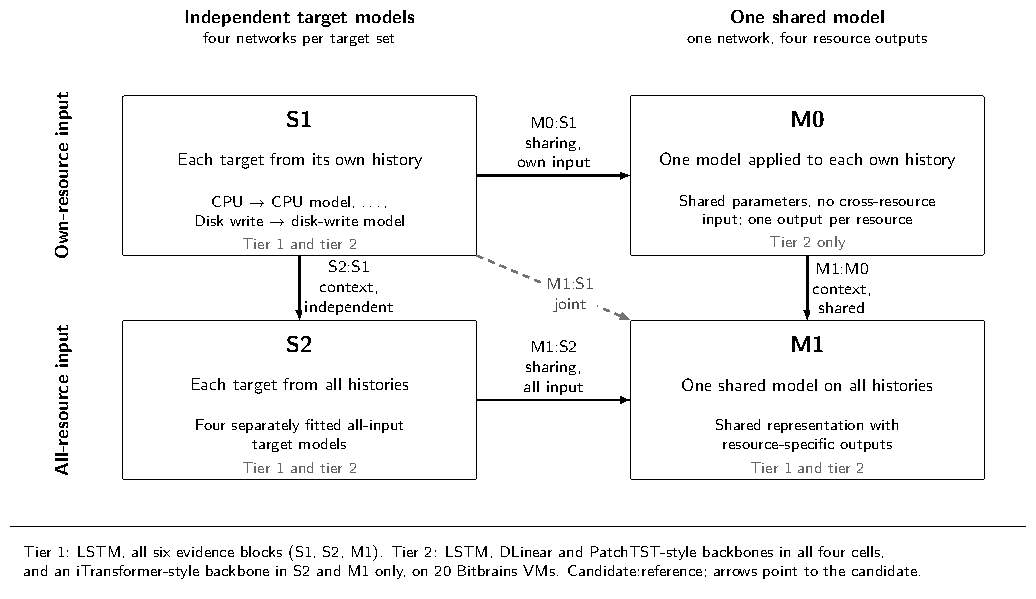
\includegraphics[width=\textwidth]{Figure_1.pdf}
  \caption{The $2\times2$ design. Rows set the input scope (own resource or
  all four resources); columns set parameter sharing (four independent target
  models or one shared model with resource-specific outputs). Vertical
  contrasts change context with sharing fixed (S2:S1, M1:M0); horizontal
  contrasts change sharing with input fixed (M0:S1, M1:S2); the dashed
  diagonal M1:S1 changes both. Models are fitted separately for each entity,
  outer fold and seed, and never shared across entities. Tier~1 evaluates
  S1, S2 and M1 with the LSTM; tier~2 adds M0 and further backbones. The
  contrasts are matched operational comparisons, not parameter-matched
  interventions or pure causal isolation of either decision.}
  \label{fig:sharing-framework}
\end{figure*}

\subsection{Problem Formulation}
\label{sec:problem}

Let $\mathcal{R}=\{\mathrm{cpu},\mathrm{thr},\mathrm{mem},\mathrm{disk}\}$
denote the resource set and let $R=|\mathcal{R}|=4$. At discrete time $t$,
the multivariate telemetry observation is
$\mathbf{x}_t=(x_t^{(r)})_{r\in\mathcal{R}}\in\mathbb{R}^{R}$. For a context
length $L\in\mathbb{N}$, the complete history available at forecasting origin
$t$ is
\begin{equation}
  \mathbf{X}_{t,L}
  = [\mathbf{x}_{t-L+1},\ldots,\mathbf{x}_{t}]^{\mathsf T}
  \in \mathbb{R}^{L\times R}.
  \label{eq:multiresource-context}
\end{equation}
Let $\mathcal{H}\subset\mathbb{N}_{>0}$ be a finite set of forecast horizons.
For target resource $r$, $y_{t+h}^{(r)}$ is the future target at horizon
$h\in\mathcal{H}$ and
$\mathbf{y}_{t,\mathcal{H}}^{(r)}=(y_{t+h}^{(r)})_{h\in\mathcal{H}}$ is its
multi-horizon target vector. A forecaster produces
\begin{equation}
  \widehat{\mathbf{y}}_{t,\mathcal{H}}^{(r)}
  = F_r(\mathcal{I}_{t,L};\boldsymbol{\theta}),
  \label{eq:forecasting-task}
\end{equation}
where $\mathcal{I}_{t,L}$ denotes the formulation-dependent information set
and $\boldsymbol{\theta}$ denotes the relevant model parameters.

Models are entity-specific: for each machine or VM, outer fold and seed, S1/S2
fit four target-specific networks and M1 (and, in tier~2, M0) one joint
four-resource network, never shared across entities. Contexts contain
observations available at or before $t$; targets lie strictly afterwards, and
matched origins, targets, horizons and partitions prevent sample differences
from changing a contrast. The four resources are CPU utilisation, aggregate
throughput, memory usage and disk-write activity, and every formulation
predicts its full horizon vector directly.

\subsection{Four Formulations}
\label{sec:formulations}
\label{sec:s1}
\label{sec:s2}
\label{sec:m1}
\label{sec:m0}

S1 gives each target resource $r$ its own model on its own history,
\begin{equation}
  \mathbf{X}_{t,L}^{\mathrm{S1},r}
  = [x_{t-L+1}^{(r)},\ldots,x_t^{(r)}]^{\mathsf T}
  \in\mathbb{R}^{L\times 1},
  \label{eq:s1-input}
\end{equation}
and its output is
\begin{equation}
  \widehat{\mathbf{y}}_{t,\mathcal{H}}^{(r)}
  = f_r^{\mathrm{S1}}
    (\mathbf{X}_{t,L}^{\mathrm{S1},r};\boldsymbol{\theta}_r^{\mathrm{S1}})
  \in\mathbb{R}^{|\mathcal{H}|}.
  \label{eq:s1-forecast}
\end{equation}
S2 gives each target its own model on all four histories,
\begin{equation}
  \mathbf{X}_{t,L}^{\mathrm{S2},r}=\mathbf{X}_{t,L}
  \in\mathbb{R}^{L\times R},
  \qquad
  \widehat{\mathbf{y}}_{t,\mathcal{H}}^{(r)}
  = f_r^{\mathrm{S2}}
    (\mathbf{X}_{t,L};\boldsymbol{\theta}_r^{\mathrm{S2}}).
  \label{eq:s2-forecast}
\end{equation}
so non-target histories act as covariates, but gradients from one target
cannot update another target's model. M1 combines all-resource input with an
encoder shared across targets and resource-specific heads:
\begin{equation}
  \begin{aligned}
    \mathbf{z}_t
      &= E_{\boldsymbol{\theta}}(\mathbf{X}_{t,L}), \\
    \widehat{\mathbf{y}}_{t,\mathcal{H}}^{(r)}
      &= g_{r,\boldsymbol{\phi}_r}(\mathbf{z}_t),
      && r\in\mathcal{R}.
  \end{aligned}
  \label{eq:m1-forecast}
\end{equation}
Let $\mathcal{B}$ be a training mini-batch, and let
$\widetilde{y}_{i,h}^{(r)}$ and
$\widehat{\widetilde{y}}_{i,h}^{(r)}$ denote the scaled target and prediction
for sample $i$, resource $r$, and horizon $h$. M1 uses the equally weighted
scaled-space objective
\begin{equation}
  \mathcal{L}_{\mathrm{M1}}
  = \frac{1}{|\mathcal{B}|R|\mathcal{H}|}
    \sum_{i\in\mathcal{B}}
    \sum_{r\in\mathcal{R}}
    \sum_{h\in\mathcal{H}}
    \left(
      \widehat{\widetilde{y}}_{i,h}^{(r)}
      - \widetilde{y}_{i,h}^{(r)}
    \right)^2.
  \label{eq:m1-loss}
\end{equation}
Equal coefficients do not imply equal realised losses or gradients, and no
task weights are learned. M0 applies one shared forecaster to each resource's
own history,
\begin{equation}
  \widehat{\mathbf{y}}_{t,\mathcal{H}}^{(r)}
  = g_{r,\boldsymbol{\phi}_r}\!\left(
      E_{\boldsymbol{\theta}^{\mathrm{M0}}}
      (\mathbf{X}_{t,L}^{\mathrm{S1},r})\right),
  \qquad r\in\mathcal{R}.
  \label{eq:m0-forecast}
\end{equation}
trained with the same objective; it is evaluated only in tier~2, with
backbone-specific forms in Section~\ref{sec:tier2-design}. Supplementary
Section~S-B0 gives the full formulation text.

\subsection{Controlled Information-Sharing Decomposition}
\label{sec:decomposition}

The matched operational formulations define comparisons, each evaluated for the same
resource, horizon, and matched support. Let $Q(F)$ denote a lower-is-better
error functional for formulation $F$ under such a fixed evaluation unit. For
a baseline $A$ and candidate $B$, define the signed error reduction
\begin{equation}
  D_Q(A\rightarrow B)=Q(A)-Q(B),
  \label{eq:controlled-reduction}
\end{equation}
so that a positive value indicates lower error for $B$. Exact metric,
aggregation, and percentage-normalisation rules are specified in the
experimental methodology. The framework-level contrasts are
\begin{equation}
  \begin{aligned}
    \mathcal{C}_{\mathrm{context}}
      &= D_Q(\mathrm{S1}\rightarrow\mathrm{S2}), \\
    \mathcal{C}_{\mathrm{sharing}}
      &= D_Q(\mathrm{S2}\rightarrow\mathrm{M1}), \\
    \mathcal{C}_{\mathrm{joint}}
      &= D_Q(\mathrm{S1}\rightarrow\mathrm{M1}).
  \end{aligned}
  \label{eq:controlled-contrasts}
\end{equation}

None presumes an error ordering, and native-unit errors are never averaged
across resources. On matched support the S1-to-M1 raw difference equals the
sum of its two intermediate differences, without implying mechanistic
additivity; percentages are not additive because each uses its own reference.

The tier-2 $2\times2$ adds one contrast for each decision with the other
held at its alternative level:
\begin{equation}
  \begin{aligned}
    \mathcal{C}_{\mathrm{context}\mid\mathrm{shared}}
      &= D_Q(\mathrm{M0}\rightarrow\mathrm{M1}), \\
    \mathcal{C}_{\mathrm{sharing}\mid\mathrm{own}}
      &= D_Q(\mathrm{S1}\rightarrow\mathrm{M0}).
  \end{aligned}
  \label{eq:tier2-contrasts}
\end{equation}
S1 and M1 are then connected by two paths, through S2 and through M0, with
the same raw total. Whether the two decisions interact is described by the
entity log-ratio
\begin{equation}
  I=\ln A_{\mathrm{M1}}-\ln A_{\mathrm{S2}}-\ln A_{\mathrm{M0}}
    +\ln A_{\mathrm{S1}},
  \label{eq:interaction}
\end{equation}
where $A_X$ is an entity's MacroMAE for cell $X$ over its folds and horizons.
$I>0$ means sharing costs more, in log-error terms, with all-resource input
than with own-resource input. $I$ is reported descriptively, not tested.

\section{Experimental Methodology}
\label{sec:methodology}

The formulations in Section~\ref{sec:framework} are retained across one
development dataset, two external environments and three dependent temporal
blocks, adapting source-specific fields and sample offsets.

\subsection{Research Questions}
\label{sec:research-questions}

Six research questions use the matched contrasts in
Section~\ref{sec:decomposition}. Each is answered separately for the two
tiers where both apply.

\begin{description}
  \item[RQ1:] How do the backbones compare in baseline accuracy (tier~2
    MacroMAE and persistence skill on common units)?
  \item[RQ2:] When does contextual input help? S2:S1 in both tiers, and M1:M0
    with sharing held fixed in tier~2.
  \item[RQ3:] When does representation sharing hurt? M1:S2 in both tiers, and
    M0:S1 with own-resource input and their interaction
    (Equation~\ref{eq:interaction}) in tier~2; the joint change M1:S1 is
    reported here too.
  \item[RQ4:] Which diagnostics accompany the sharing cost (dependence,
    gradient conflict and magnitude, loss shares and transfer for the tier-2
    LSTM), and does loss balancing reduce it (A1)?
  \item[RQ5:] How stable are the effects across resources, environments,
    temporal blocks and evaluation units, and what accuracy--consolidation
    trade-offs arise?
  \item[RQ6:] Can the inner-validation errors available before deployment
    decide consolidation (A3)?
\end{description}

These specify estimands, not expected benefits. Supplementary Section~S-E
maps them to the tier-1 protocol's numbering.

\subsection{Data, Targets and Leakage Control}
\label{sec:datasets}
\label{sec:preprocessing}
\label{sec:leakage-control}
\label{sec:population-restrictions}
\label{sec:replication-design}

Table~\ref{tab:dataset-summary} summarises the sources. TimeTrack, telemetry
from the OpenAirInterface (OAI) CI/CD system on seven machines between
24 June and 19 July 2024, is framework-development evidence with a measured
median sampling interval of about 42.3 seconds; gaps longer than twice that
interval start a new segment. The Bitbrains fastStorage and Rnd traces are two separate
external environments with five-minute sampling, in which physically invalid
rows are removed and gaps longer than 450 seconds delimit segments. Materna
T1--T3 are consecutive, dependent blocks from one source on a 300-second grid
and provide secondary temporal replication, not independent datasets. All
sources map to CPU, throughput, memory and disk write: CPU and memory use the
identity transform and throughput and disk write use $\log(1+x)$; each
transformed series is robust-scaled with training-only median and
interquartile range, which must be positive (no epsilon or fallback), and is
returned to native units with a non-negativity projection for throughput and
disk write.

External eligibility requires structural validity and a positive
transformed-resource interquartile range in every required training
partition. From each eligible pool, 35 VMs were selected by ascending SHA-256
rank of a fixed key, without outcome information; for Materna, 74 VMs passed
the joint rule and the first 35 are used in all three blocks. The cohorts
therefore represent scale-estimable, structurally eligible VMs, not every
archived VM.

An origin is legal only when the maximum context and every future target lie
in one contiguous segment, and common support is built at the largest
context, so all formulations share origins, targets, folds, horizons and
seeds. Five expanding outer folds use the first half of the ordered legal
origins before the first of five successive ten-percent test blocks, and
training origins whose maximum-horizon target reaches the test block are
purged. The latest 15\% of outer-training origins form inner validation,
purged again; scalers, contexts and epochs use only training and validation
data, and each final model is refitted once on the complete outer-training
support and evaluated once on its test block. Horizons are
$\{1,2,4,8,16,32,64,128\}$ samples in TimeTrack (about 0.7 to 90
minutes) and $\{1,2,4,9,18\}$ samples externally (5, 10, 20, 45 and 90
minutes), with candidate contexts of 32, 64 and 128 and of 4, 9 and 18
samples. Bitbrains environments and Materna blocks are analysed separately
before any equal-weight descriptive summary, and no score pools sources.
Supplementary Section~S-B1 gives the full data, preprocessing and leakage
protocol.

\begin{table*}[t]
  \caption{Evidence sources, study roles and prespecified protocol adaptations,
  distinguishing eligible populations from executed cohorts. Materna T1--T3
  are dependent temporal blocks.}
  \label{tab:dataset-summary}
  \centering
  \small
  \setlength{\tabcolsep}{3pt}
  \begin{tabular}{@{}
    >{\raggedright\arraybackslash}p{0.110\textwidth}
    >{\raggedright\arraybackslash}p{0.110\textwidth}
    >{\raggedright\arraybackslash}p{0.195\textwidth}
    >{\raggedright\arraybackslash}p{0.225\textwidth}
    >{\raggedright\arraybackslash}p{0.100\textwidth}
    >{\raggedright\arraybackslash}p{0.195\textwidth}@{}}
    \toprule
    Source / block & Study role & Temporal structure / cadence
      & Eligibility & Executed cohort & Forecast protocol \\
    \midrule
    TimeTrack & Framework development
      & 42.3 s median; 9 gap-bounded segments
      & Seven machines; 41,356-row canonical panel
      & 7 machines & 0.7--90.2 min (eight leads) \\
    \addlinespace
    Bitbrains fastStorage & External confirmation
      & Separate environment; 5 min; per-VM segments
      & 916/1,250 structural; 596/916 scale eligible
      & 35 VMs & 5, 10, 20, 45, 90 min (five leads) \\
    \addlinespace
    Bitbrains Rnd & External confirmation
      & Separate environment; 5 min; per-VM segments
      & 416/500 structural; 272/416 scale eligible
      & 35 VMs & 5, 10, 20, 45, 90 min (five leads) \\
    \addlinespace
    Materna T1--T3 & Secondary replication
      & 5 min; blocks analysed separately
      & 398 common structural; 74/398 all-block scale
      & 35 shared VMs & 5, 10, 20, 45, 90 min (five leads) \\
    \bottomrule
  \end{tabular}

  \vspace{2pt}
  \parbox{\textwidth}{\footnotesize
    All experiments forecast CPU utilisation, throughput, memory usage and
    disk-write activity. Materna provides secondary temporal replication:
    T1--T3 are consecutive dependent blocks from the same source and selected
    cohort, not independent datasets.}
\end{table*}


\subsection{Models, Training and Selection}
\label{sec:architecture-training}
\label{sec:model-selection}

Tier~1 uses a plain two-layer unidirectional LSTM \citep{Hochreiter1997LSTM}
with hidden size 64 and dropout 0.1. S1 and S2 minimise target-specific scaled
mean squared error and M1 the mean of the four resource-specific errors
(Equation~\ref{eq:m1-loss}). Training uses Adam with learning rate 0.001,
batch size 256, at most 50 epochs, early-stopping patience 7, gradient-norm
clipping at 1.0 and seeds 0, 1 and 2, with no architecture or optimiser
search. Context length is selected from the candidate grid on
inner-validation scaled MAE at each seed's MSE-selected epoch, per target for
S1 and S2 and per entity and fold for M1, and exact ties favour the shorter
context; each final model is refitted with the selected context and
seed-specific epoch count. In the five-horizon external design the
complements have 203,028 (S1), 206,100 (S2) and 52,500 (M1) parameters.
Reported fit time sums successful worker fit-hours and is not elapsed wall
time, energy or deployment cost (Supplementary Section~S-B2).

\subsection{Evaluation and Uncertainty}
\label{sec:evaluation}

Primary evaluation uses native-unit MAE after inverse transformation and
projection; native errors are never averaged across different resources, and
RMSE, $R^2$ and native NMAE were recorded but are not analysed here. Persistence supplies a
separate absolute forecasting check:
\begin{equation}
  \widehat{y}_{t+h}^{(r),\mathrm{pers}}=y_t^{(r)},
  \qquad
  \operatorname{Skill}_{r,h}
  =1-\frac{\operatorname{MAE}_{r,h}^{\mathrm{model}}}
           {\operatorname{MAE}_{r,h}^{\mathrm{pers}}}.
  \label{eq:persistence-skill}
\end{equation}
averaged over entity--fold cells and then horizons, with undefined
zero-denominator skills excluded and counted. MAE is averaged over the three
seeds within each matched entity, fold, resource, horizon and formulation
cell; for a fixed resource and horizon, seed-averaged cells receive equal
weight to form MacroMAE, and a resource-overall MacroMAE gives equal weight to
every horizon. For candidate $C$ and baseline $B$, the reported gain is
\begin{equation}
  G(C\!:\!B)=100\,
  \frac{\operatorname{MacroMAE}(B)-\operatorname{MacroMAE}(C)}
       {\operatorname{MacroMAE}(B)}.
  \label{eq:macro-gain}
\end{equation}
A positive value indicates lower candidate error.  The three tier-1
contrasts are S2 versus S1, M1 versus S2, and M1 versus S1; tier~2 adds M1
versus M0 and M0 versus S1. Because native-unit cells receive equal weight
without rescaling across entities, an entity whose resource is on a much
larger native scale can dominate MacroMAE and hence $G$. Matched-cell median
ratios, win rates and per-entity signs are unaffected by this scale
weighting and are reported alongside. The Results lead with these
typical-machine statistics because native-unit aggregation lets a single
high-scale VM set a gain; this emphasis was chosen after the results were
known, and the prespecified MacroMAE gains remain reported in full
(Supplementary Section~S-G). Secondary descriptives are the counts of
positive VMs, folds, horizons and seed aggregates.

Prespecified classes---\textsc{Broad Positive},
\textsc{Conditionally Positive}, \textsc{Broad Negative} and
\textsc{Neutral or Mixed}---combine the overall gain (at least $+1\%$,
strictly positive, or at most $-1\%$) with consistency over horizons,
entities, folds and seeds; the thresholds are in Supplementary
Section~S-B3 and the supplementary decision criteria. Intervals never enter
the classes, and no threshold is adapted after observing outcomes. External
uncertainty uses a paired VM-cluster bootstrap within each Bitbrains
environment and Materna trace that samples 35 VMs with replacement, retains
all five folds and the paired formulation structure, and uses 10,000
replicates, percentile 95\% intervals and random seed 20261007. TimeTrack has
no such intervals.

\subsection{Post-Hoc Sensitivity Analyses}
\label{sec:posthoc-controls}

Three analyses were added after the tier-1 experiment was frozen. They are
post-hoc sensitivity controls, not amendments to the prospective design or
replacements for its results, and retain the tier-1 cohorts, folds, horizons,
purging, support, transforms, scalers and native-unit evaluation.
\emph{Common-context S2} imposes the selected H64-M1 context on every S2 target,
removing S2's context-selection freedom. \emph{H129 M1} raises the shared
hidden size from H64 to H129 (206,420 parameters externally), approximately
matching the 206,100-parameter S2 complement, with selection repeated afresh.
\emph{Matched-context Ridge AR/ARX} compares own-lag and all-resource-lag
Ridge models at the H64-M1 context, with $\alpha$ selected on inner
native-unit validation MAE. Neither LSTM control equalises architecture or
optimisation, and Ridge tests input scope in a second model family rather
than isolating model family (procedures in Supplementary Section~S-B4).

AI-assisted analysis code (see the declaration at the end) was inspected,
tested and validated by the authors against the frozen artifacts before use;
generative AI did not generate or modify experimental observations or reported
results.

\subsection{Tier-2 Design}
\label{sec:tier2-design}

Tier~2 is the separately frozen part of the study that completes the $2\times2$ design
and repeats it across backbone families. It reuses, without refitting, every
tier-1 result and post-hoc control above, and it changes no tier-1 estimand.

\paragraph{Cohort and data} Tier~2 uses 20 Bitbrains VMs: the first ten per
environment by the fixed cohort rank, chosen by rank rather than outcome
(fastStorage 697, 860, 366, 679, 360, 505, 481, 109, 680, 50; Rnd 99, 409,
269, 493, 474, 97, 118, 233, 142, 151). Origins, legal support, the five
purged expanding outer folds, horizons $\{1,2,4,9,18\}$, source-specific
transforms, training-only scalers, inverse transformation, non-negativity
projection and native-unit test origins are those of tier~1, and inputs are
byte-identical to the archived inputs. Each outer fold has one inner
training and validation split. Every backbone and cell uses the tier-1 H64-M1
context $L\in\{4,9,18\}$ for each entity and fold, with no new context
selection; the tier-2 LSTM S1 and S2 fits therefore differ from tier~1, which
selected contexts per target. All four LSTM cells are refitted with one
pipeline so that the $2\times2$ is not confounded by mixing pipelines.

\paragraph{Backbones} Hyperparameters are fixed in advance and identical
across cells except where a cell's definition requires otherwise (learning
rate $10^{-3}$, batch size 256, at most 50 inner epochs, patience 7, clipping
at 1.0, seeds 0--2), with no hyperparameter search. The LSTM is as in tier~1,
with M0 an input-size-one encoder shared across the four own-resource
histories. DLinear \citep{Zeng2023DLinear} forecasts trend and residual
components with linear maps: its M0 reuses one pair of maps on every
resource channel without resource-specific outputs, S2 is a decomposed linear
ARX, and M1 passes all inputs through a shared linear bottleneck of width 16
before per-target heads. The PatchTST-style backbone \citep{Nie2023PatchTST}
applies one patch Transformer to each channel in M0 and channel-dependent
tokens in S2 and M1. The iTransformer-style backbone
\citep{Liu2024iTransformer} embeds each resource history as a variate token;
its S1 and M0 cells are undefined because a single token reduces attention to
a token-wise multilayer perceptron. Both transformer-style backbones are
declared adaptations, not canonical implementations, and every new cell
passed structural checks before any data fit. Full specifications are in
Supplementary Section~S-B5.

\paragraph{Execution} All 13{,}500 final fits and outer-test evaluations
completed without retries, and no unit was missing (Supplementary
Section~S-E).

\subsection{Tier-2 Analysis and Diagnostics}
\label{sec:tier2-analysis}

\paragraph{Endpoints} Tier~2 uses the gain in
Equation~\ref{eq:macro-gain} and the consistency classes of
Section~\ref{sec:evaluation} for each backbone, contrast, resource and
block, with seed thresholds unchanged and VM thresholds rescaled to ten VMs
by rounding conservatively: at least 8/10 positive VMs for
\textsc{Broad Positive}, at least 5/10 for \textsc{Conditionally Positive}
and at most 2/10 for \textsc{Broad Negative}, with horizon thresholds 4/5,
3/5 and 1/5. A fit that failed after its permitted retries would have made
the corresponding unit missing for every cell of that backbone, keeping
contrasts paired; none failed. Matched-cell median ratios, win rates,
persistence skill and parameter counts are reported as descriptives.
Backbones are compared on their common available units.

\paragraph{Uncertainty and cross-backbone summary} The bootstrap of
Section~\ref{sec:evaluation} resamples each block's ten VMs, with one draw
matrix per block, generated in the order fastStorage then Rnd, reused for
every interval in that block. An effect \emph{generalises across backbones} only
if every backbone for which the contrast is defined has a non-neutral class
of the same sign; otherwise it is \emph{backbone-dependent}. No pooled
cross-backbone statistic is computed.

\paragraph{Diagnostics} Seven diagnostics are computed on the same cohort,
after all fits had finished for training-side measures and after all
evaluations had finished for anything involving outcomes; none alters a model.
D-1 is the maximum absolute lagged cross-correlation (lags 1--18) between
ordered resource pairs on inner-training series; D-2 reuses the post-hoc Ridge
ARX:AR gain; D-3 is the Spearman correlation across the ten VMs of each block
between D-1 or D-2 and the LSTM entity log effects
$D(C\!:\!B)=\ln A_C-\ln A_B$; D-4 measures, in the LSTM M1 shared encoder at
the selected epoch over eight keyed batch pairs, the pairwise task-gradient
cosines, the ratio of the largest to the smallest task-gradient norm and the
excess sign-conflict rate $K$; D-5 fits all-input LSTM models on pairwise and
leave-one-out resource subsets, from which D-6 derives directed transfer
$F_i(j)$ and leave-one-out contribution $Q_{i,j}$ (positive values favour
adding or retaining resource $j$); and D-7 is each task's share of the M1
training loss. Definitions are in Supplementary Section~S-B6.
They are descriptive associations, reported whatever their direction, and
change no other component. No intervention, such as a
robust loss or gradient surgery, is fitted except loss balancing (A1); A3
evaluates validation-selected grouping of already fitted models.

\subsection{Loss-Balancing Amendment (A1)}
\label{sec:a1-design}

The diagnostics motivated one intervention, added as amendment A1 after the
tier-2 results were known and frozen before any A1 fit. Tier~2's records were
already closed to new fits, so A1 was run as its own package, fixed by its own
Git tag. It reuses the tier-2
cohort, folds, contexts, scalers, LSTM architecture and training settings,
and it reads the tier-2 equal-loss M1, S2 and S1 outcomes without refitting
them. The hypothesis was stated in advance: \emph{equalising the tasks'
contributions to the shared encoder's training reduces the shared LSTM's
typical-cell accuracy penalty, compared with the equal-weight loss.}

Only the training loss of the shared all-input LSTM changes. M1-GN (primary)
applies GradNorm \citep{Chen2018GradNorm} to the second LSTM layer, with
$\alpha=1.5$ and task weights summing to four. M1-UW (secondary) applies
uncertainty weighting, $\sum_i (e^{-s_i}L_i+s_i)$ with learnable $s_i$
\citep{Kendall2018Uncertainty}. Settings were fixed without tuning, epoch
selection still uses the unweighted equal-mean validation error, and each A1
fit starts from the same initialisation and batch order as its tier-2 M1 fit.

The primary endpoint is the matched-cell median ratio and win rate against
equal-loss M1 in each of the eight resource $\times$ block cells. An arm is
\emph{supported} if it beats M1 (ratio below one and win rate above 0.5) in
at least six cells and its effective task-gradient norm ratio is below M1's
in both blocks; the effective ratio uses each task's D-4 norm times its
training weight. An arm \emph{removes the penalty} if, in addition, its ratio
against S2 is at most one in at least six cells. MacroMAE gains, classes and
intervals are reported but do not enter the rule. All 1{,}200 A1 fits, 600
gradient extractions and 600 evaluations completed, and no unit was missing
(Supplementary Section~S-F).

\subsection{Validation-Gate Amendment (A3)}
\label{sec:a3-design}

A3 tests whether consolidation can be decided before deployment, from the
inner-validation errors every fit had recorded (scaled MAE in tier~1, scaled
MSE in tier~2). It fits no model. It was specified after all other results
were known and frozen by its own Git tag before any of its outcomes was
computed, so it tests decision rules, not the component models. For each
machine, fold and seed, G-share($\tau$) replaces the four S2 models by M1 when
the mean validation ratio M1/S2 over the resources is at most $1+\tau$
($\tau\in\{0,0.5,1,2\}\%$; $1\%$ primary). For the tier-2 LSTM, G-group($\tau$)
picks, among the 15 groupings of the four resources built from S2, M1 and the
pair and triple models of diagnostic D-5, the feasible grouping with the
fewest models. A fallback to persistence and an outer-test oracle are
secondary. The frozen rules ask whether the gate keeps at least half of the
model saving with at most half the M1:S2 cost cells (median ratio above
1.01), whether validation and outer M1/S2 ratios are rank-correlated
($\rho\geq0.3$, interval above zero), and whether grouping saves at least 0.25
models per unit more than G-share (Supplementary Section~S-H).

\subsection{Validation Strategy}
\label{sec:validation-strategy}

Each threat is met by a named mechanism; those added after results were known
are labelled post hoc. \emph{Leakage:} chronological purged expanding folds, a purged inner
validation split, and training-only scalers, contexts and epochs
(Section~\ref{sec:datasets}); tier-2 outer-test data were not read until all
fits had finished. \emph{Sample mismatch:} every formulation shares origins,
targets, folds, horizons and seeds, and a failed fit would remove its unit
from every cell of the backbone (Section~\ref{sec:tier2-analysis}).
\emph{Selection freedom:} the tier-1 external criteria were prospective,
and tier~2, A1 and A3 were each frozen by an annotated Git tag and package
digest, with an execution seal where models were fitted, before any of their
outcomes. \emph{Context and capacity:} the common-context S2 and
capacity-matched H129 M1 controls; \emph{model family:} Ridge AR/ARX and four
tier-2 backbones (Sections~\ref{sec:posthoc-controls}
and~\ref{sec:tier2-design}). \emph{Scale dominance:} matched-cell median
ratios and win rates beside MacroMAE (Section~\ref{sec:evaluation}).
\emph{VM sampling:} paired VM-cluster bootstrap intervals. \emph{Seed
variation:} three seeds, with sign changes reported. \emph{Implementation
error:} structural checks of every new cell, one pipeline for all LSTM cells,
byte-identical inputs, a read-only audit of the largest aggregate, and
figures, tables and A3 numbers generated by scripts that verify the output
digests. \emph{Absolute accuracy:} persistence skill. \emph{Mechanism and
decision:} A1, with a manipulation check, and A3.

Resampling VMs rather than observations keeps the serial and cross-horizon
dependence within a machine inside each resample. No hypothesis tests are
performed, so no multiplicity correction applies: effects are judged by
prespecified classes that require consistency across horizons, VMs, folds and
seeds. The $1\%$ margin used in the text is descriptive and
matches the class gain threshold. A Git tag, package digest and seal make the
frozen protocol, code and inputs verifiable, but, unlike a time-stamped
registry entry, do not prove when they were frozen.
Supplementary Table~S26 maps each main claim to its evidence and its limits.

\section{Results}

Each result is given first for a typical machine: the median, over matched
entity $\times$ fold $\times$ horizon cells, of the candidate/reference MAE
ratio with MAE averaged over seeds, and the candidate's win rate
(Figures~\ref{fig:primary-gains} and~\ref{fig:tier2-contrasts}). The
prespecified MacroMAE gains follow (full values, classes and intervals:
Supplementary Section~S-G and Table~S3); post-hoc controls are in
Table~\ref{tab:posthoc-controls} and Supplementary Tables~S1--S2.

\begin{figure*}[t]
\centering
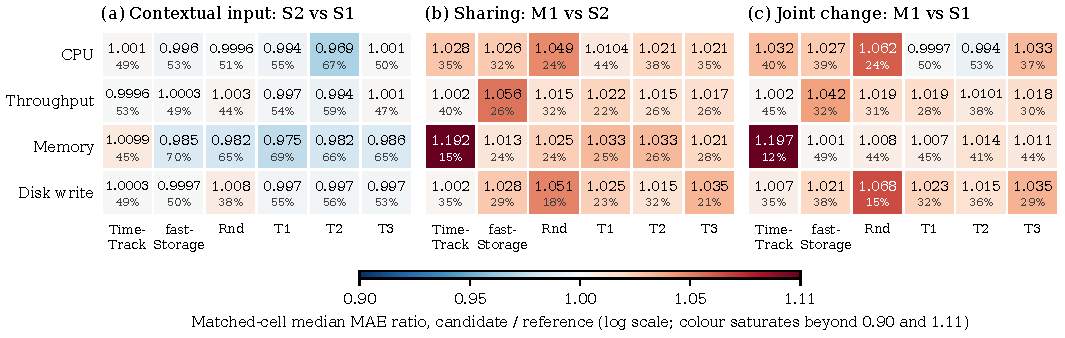
\includegraphics[width=\textwidth]{Figure_2.pdf}
\caption{Tier~1 for a typical machine: median matched-cell MAE ratio,
candidate/reference (large number and colour), and the candidate's win rate
(small number) for (a) S2 versus S1, (b) M1 versus S2 and (c) M1 versus S1.
A cell is entity $\times$ outer fold $\times$ lead, with MAE averaged over
the three seeds. A ratio below one and a win rate above $50\%$ favour the
candidate. These are post-hoc descriptives of the prespecified comparisons;
(c) is computed in the same way from the same cells. T1--T3 are the dependent
Materna temporal blocks. Colour saturates beyond 0.90 and 1.11; printed values
are authoritative. Prespecified MacroMAE gains: Supplementary Section~S-G.}
\label{fig:primary-gains}
\end{figure*}

\subsection{RQ1 Backbone Baseline Accuracy}
\label{sec:results-baselines}

On the 20 Bitbrains VMs, no backbone was most accurate throughout, and none
beat persistence for CPU or throughput. Table~\ref{tab:tier2-baseline} places the LSTM beside the
DLinear, PatchTST-style and iTransformer-style backbones on common units. Outside
fastStorage CPU, the LSTM's MacroMAE was within a factor of 1.04 of the most
accurate defined backbone in every cell (S1, S2, M0 and M1) and resource, and
it was the most accurate S2 backbone for Rnd CPU, memory and disk write.
fastStorage CPU was the exception: DLinear was most accurate in every cell,
and the LSTM's MacroMAE was 1.89--2.17 times DLinear's. Persistence skill separates the resources rather than
the backbones: CPU and throughput skill was negative for every backbone and
cell in both blocks, whereas memory and disk-write skill was positive. These
are descriptive comparisons under one imposed context and fixed
hyperparameters, not a ranking of architectures.


\begin{table*}[t]
  \caption{Tier-2 baseline accuracy on the 20-VM Bitbrains cohort: (A) each backbone's resource-overall MacroMAE divided by the smallest MacroMAE among the defined backbones in that row (1.00 marks the most accurate); (B) mean persistence skill. Descriptive only.}
  \label{tab:tier2-baseline}
  \centering
  \small
  \setlength{\tabcolsep}{3pt}
  \begin{tabular*}{\textwidth}{@{\extracolsep{\fill}}llrrrrrrrr@{}}
    \toprule
    \multicolumn{10}{l}{\textbf{A:} MacroMAE ratio to the most accurate backbone} \\
    & & \multicolumn{4}{c}{S2 (all input, independent)} & \multicolumn{4}{c}{M1 (all input, shared)} \\
    \cmidrule(lr){3-6}\cmidrule(l){7-10}
    Block & Resource & LSTM & DLinear & PatchTST & iTrans. & LSTM & DLinear & PatchTST & iTrans. \\
    \midrule
    fastStorage & CPU & 1.99 & \textbf{1.00} & 1.97 & 1.96 & 1.89 & \textbf{1.00} & 1.86 & 1.77 \\
     & Throughput & 1.02 & \textbf{1.00} & 1.04 & 1.03 & 1.02 & 1.11 & \textbf{1.00} & 1.01 \\
     & Memory & \textbf{1.00} & 1.00 & 1.02 & 1.02 & \textbf{1.00} & 1.04 & 1.01 & 1.01 \\
     & Disk write & 1.03 & \textbf{1.00} & 1.02 & 1.02 & 1.01 & \textbf{1.00} & 1.02 & 1.02 \\
    Rnd & CPU & \textbf{1.00} & 1.03 & 1.09 & 1.01 & 1.01 & 1.11 & 1.05 & \textbf{1.00} \\
     & Throughput & 1.01 & 1.13 & 1.06 & \textbf{1.00} & 1.03 & 1.16 & 1.05 & \textbf{1.00} \\
     & Memory & \textbf{1.00} & 1.04 & 1.05 & 1.02 & 1.03 & 1.01 & \textbf{1.00} & 1.00 \\
     & Disk write & \textbf{1.00} & 1.07 & 1.04 & 1.01 & 1.04 & 1.02 & 1.03 & \textbf{1.00} \\
    \midrule
    \multicolumn{10}{l}{\textbf{B:} Mean persistence skill} \\
    & & \multicolumn{4}{c}{S2 (all input, independent)} & \multicolumn{4}{c}{M1 (all input, shared)} \\
    \cmidrule(lr){3-6}\cmidrule(l){7-10}
    Block & Resource & LSTM & DLinear & PatchTST & iTrans. & LSTM & DLinear & PatchTST & iTrans. \\
    \midrule
    fastStorage & CPU & $-$0.70 & $-$0.16 & $-$0.76 & $-$0.85 & $-$0.75 & $-$0.20 & $-$0.85 & $-$0.79 \\
     & Throughput & $-$0.14 & $-$0.20 & $-$0.20 & $-$0.16 & $-$0.25 & $-$0.66 & $-$0.25 & $-$0.28 \\
     & Memory & +0.19 & +0.18 & +0.18 & +0.18 & +0.18 & +0.12 & +0.17 & +0.18 \\
     & Disk write & +0.27 & +0.29 & +0.26 & +0.28 & +0.25 & +0.25 & +0.22 & +0.25 \\
    Rnd & CPU & $-$0.30 & $-$0.09 & $-$0.46 & $-$0.43 & $-$0.48 & $-$0.29 & $-$0.59 & $-$0.49 \\
     & Throughput & $-$0.04 & $-$0.07 & $-$0.11 & $-$0.14 & $-$0.09 & $-$0.13 & $-$0.24 & $-$0.16 \\
     & Memory & +0.17 & +0.16 & +0.16 & +0.17 & +0.12 & +0.12 & +0.13 & +0.15 \\
     & Disk write & +0.28 & +0.22 & +0.24 & +0.27 & +0.18 & +0.18 & +0.16 & +0.22 \\
    \bottomrule
  \end{tabular*}

  \vspace{2pt}
  \parbox{\textwidth}{\footnotesize Ten VMs per block, three seeds, tier-1 H64-M1 contexts imposed on every backbone, fixed untuned hyperparameters. iTransformer is defined only for S2 and M1. Backbones are compared on their common available units (no unit was missing). S1 and M0 rows are in the supplement.}
\end{table*}


\subsection{RQ2 Contextual Input}
\label{sec:results-rq1}

Contextual input helped selectively. In tier~1
(Figure~\ref{fig:primary-gains}(a)), memory showed the only recurring
benefit: the all-input model S2 was more accurate than S1 in typical cells in
all five external blocks (median ratios 0.975--0.986, win rates
$65$--$70\%$), though not on TimeTrack (1.0099). For the other resources the
median ratios stayed between 0.969 and 1.008. In MacroMAE terms, memory was
broadly positive in fastStorage and Materna T2, conditionally positive in Rnd
and T3, the sole positive resource on TimeTrack and slightly negative in T1
($-0.02\%$); the two views differ only where both effects are near zero. The
other resources changed direction across blocks, Rnd throughput and T1 disk
write being adverse where other blocks were near zero or positive, and many
intervals crossed zero. The matched-context Ridge
ARX:AR comparison also showed selective, family-dependent value: memory
improved under Ridge in all five external blocks but reversed in TimeTrack,
and the Ridge TimeTrack throughput gain of $-838.45\%$ is concentrated in one
machine/fold ($99.93\%$ of positive excess error) rather than a broad
failure. Existing-seed diagnostics find sign changes in 9/24 LSTM S2:S1
block/resource summaries (Supplementary Table~S2), so seed-varying point gains
are not seed-invariant improvements. Block-by-block classes, intervals and the
Ridge audit are in Supplementary Section~S-C1.

\paragraph{Tier-2 contextual input across backbones}
In tier~2 (Figure~\ref{fig:tier2-contrasts}(a)--(b)), contextual input was
equally small and mixed for the three backbones with a complete $2\times2$:
median S2/S1 ratios lay between 0.981 and 1.035, MacroMAE gains ranged from
$-9.22\%$ to $+3.97\%$, 8 of 24 backbone/resource/block cells reached a
positive class and 2 were broadly negative.
Memory was positive for the LSTM in both blocks and for DLinear in both
blocks, consistent with the tier-1 external memory pattern, but not for
PatchTST ($-0.26\%$ and $-2.95\%$). Rnd disk write was negative for all
three backbones. No context cell met the cross-backbone generalisation rule
(every defined backbone non-neutral with one sign). With sharing held fixed,
the median M1/M0 ratio was above one in 14 of 24 cells and the MacroMAE gain
negative in 17. The large positive DLinear Rnd
M1:M0 gains ($+46.18\%$ for CPU, $+13.61\%$ and $+13.74\%$ for memory and disk
write) coincide with a weak DLinear M0 reference, which is also worse than
DLinear S1 for those resources (panel c), rather than indicating strong
contextual value; DLinear M0 ties one linear map across all four resources without
resource-specific heads, and the CPU value is scale-dominated by one VM
(Section~\ref{sec:results-rq2}). Contextual value therefore depended on the
backbone as well as on the resource and environment.

\subsection{RQ3 Representation Sharing}
\label{sec:results-rq2}

Sharing cost accuracy in every tier-1 comparison for a typical machine. In
all 24 M1:S2 block/resource summaries the median MAE ratio exceeded one
(1.002--1.192; above 1.01 in 22) and the win rate was below $50\%$
(Figure~\ref{fig:primary-gains}(b); Supplementary Table~S1), including the
small positive CPU MacroMAE exceptions. The size of that cost varied. Materna T1/T3 disk-write median
ratios were approximately $1.0246/1.0347$, whereas their MacroMAE gains of
$-27.46\%/-71.30\%$ were concentrated in VM266 and VM272, which contributed
$82.10\%$ and $86.97\%$ of positive excess error. In MacroMAE terms,
throughput, memory and disk write had negative gains in all six blocks
(Supplementary Section~S-G) and CPU was positive only in TimeTrack,
fastStorage and Materna T1; Rnd and Materna T2 were broadly negative for
every resource with intervals below zero. Under both post-hoc controls, H64
M1 against common-context S2 and H129 M1 against S2, throughput, memory and
disk-write point estimates remained adverse in all six blocks
(Table~\ref{tab:posthoc-controls}), so context-selection freedom and the
tier-1 capacity difference do not explain the pattern, although the
controls do not isolate sharing as its cause. Gains change sign across seeds
in 4/24 M1:S2 summaries (Supplementary Section~S-C2).

\paragraph{Tier-2 sharing across backbones}
Figure~\ref{fig:tier2-contrasts}(d) repeats the all-input sharing contrast
for all four backbones. In typical cells, the shared model was less accurate
in 30 of 32 backbone/resource/block cells: the matched-cell median M1/S2
ratio exceeded one and the candidate win rate was below $50\%$. The size of
the cost differed by backbone. For the LSTM it was clear: the ratio exceeded
1.01 in 6 of 8 cells, and the post-hoc VM-cluster bootstrap interval of the
median ratio lay above one in 7 of 8. For the other three backbones it was
consistent in direction but mostly very small: 7 of 24 cells exceeded 1.01,
and 9 of 24 intervals lay above one, none below (Supplementary Table~S19).
MacroMAE
gains were negative in 29 of 32 cells, and all 16 Rnd cells were negative,
from $-1.51\%$ to $-33.11\%$. The three non-negative cells were
all fastStorage CPU (LSTM $+0.60\%$, PatchTST $+0.91\%$, iTransformer
$+5.48\%$), mirroring the tier-1 CPU exceptions. Twelve cells were broadly
negative and one, iTransformer fastStorage CPU, conditionally positive. The
remaining cells were neutral or mixed, so although the adverse direction
recurred across backbones, no M1:S2 cell met the cross-backbone
generalisation rule. Sharing with own input only (M0:S1,
Figure~\ref{fig:tier2-contrasts}(c)) separated the blocks: the median ratio
was above one in 11 of 12 Rnd cells, and all 12 Rnd MacroMAE gains were
negative, 8 of them broadly negative, whereas fastStorage was mixed with
five conditionally positive LSTM or PatchTST cells. The only two cells of
32 that generalised across backbones were both M0:S1 on Rnd, CPU and disk
write, broadly negative for the LSTM, DLinear and PatchTST.

The two sharing penalties differed by backbone. The entity log-ratio
interaction $I=\ln A_{\mathrm{M1}}-\ln A_{\mathrm{S2}}-\ln A_{\mathrm{M0}}
+\ln A_{\mathrm{S1}}$, averaged over VMs, was positive for the LSTM in all eight
resource/block cells, six with intervals excluding zero: the LSTM's sharing
penalty was larger with all-resource input than with own-resource input. It
was negative for DLinear Rnd CPU, memory and disk write, with upper interval
bounds at or just below zero, and close to zero for PatchTST, where one of
eight intervals narrowly excluded zero. Sharing also changed model size
differently across backbones. For one entity, fold and seed, LSTM M0 and M1
had 51{,}732 and 52{,}500 parameters against 203{,}028 for S1 and 206{,}100
for S2; PatchTST M1 had 69{,}012--69{,}908 against 272{,}148--275{,}732 for
S2, and iTransformer M1 72{,}404--73{,}300 against 274{,}196--277{,}780,
depending on context. DLinear M0 had 50--190 parameters against 200--760 for
S1, whereas DLinear M1, whose sharing is a 16-dimensional linear bottleneck,
had more parameters than S2 at contexts 4 and 9 (852 and 1{,}492 against 660
and 1{,}460) and fewer at context 18 (2{,}644 against 2{,}900).

\paragraph{Scale dominance in DLinear Rnd CPU}
The DLinear Rnd CPU M0:S1 gain of $-139.61\%$ and M1:M0 gain of $+46.18\%$
reproduce exactly under the prespecified aggregation, but their magnitudes are
dominated by one VM. MacroMAE averages native-unit MAE across VMs without
rescaling, and VM233's CPU errors are on a much larger native scale than the
cohort's (persistence MAE 8.85 against 0.04--1.40 for the other nine VMs).
VM233 contributes $98.6\%$ of the summed M0$-$S1 excess and $96.3\%$ of the
summed M0$-$M1 difference. Its M0 MAE exceeded S1 in every fold (1.9--4.6
times) and every seed (36.56--39.81 against 13.47--13.51 native units), and
its 15 M0 fits completed normally. The adverse direction is nevertheless
broad: M0 was worse than S1 for 8 of 10 VMs, at every horizon, in every fold
and in every seed, with a matched-cell median M0/S1 ratio of 1.051 and a win
rate of $0.34$; per-VM M0:S1 gains outside VM233 ranged from $-70.8\%$ to
$+14.0\%$. Outside VMs 233 and 269, per-VM seed spreads were at most 0.046
native units. The $-139.61\%$ aggregate is therefore valid under the prespecified
rule but describes VM233's scale, not a typical VM; the class and matched-cell
statistics describe the typical direction. A read-only audit of the stored fit
and evaluation records found no aggregation, persistence-skill or data error.

\begin{figure*}[t]
\centering
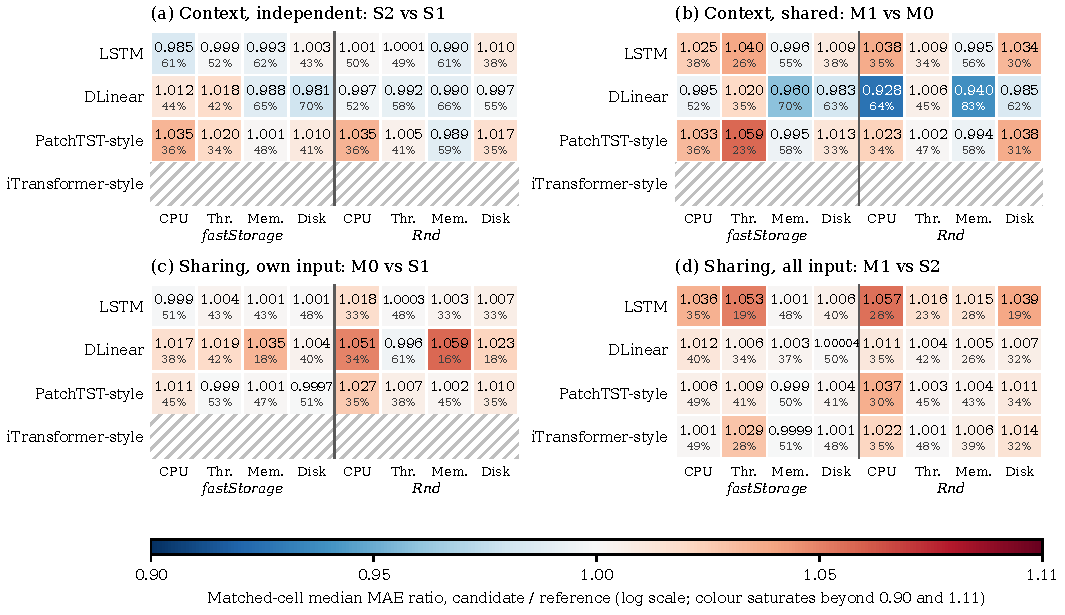
\includegraphics[width=\textwidth]{Figure_3.pdf}
\caption{Tier~2 for a typical machine on the 20-VM Bitbrains cohort:
median matched-cell MAE ratio, candidate/reference (large number and colour),
and the candidate's win rate (small number) for (a) S2 versus S1, (b) M1
versus M0, (c) M0 versus S1 and (d) M1 versus S2, by backbone, block and
resource (Thr., throughput; Mem., memory; Disk, disk write). A ratio below one
favours the candidate. Hatched cells are undefined by design (iTransformer has
no S1 or M0). Colour saturates beyond 0.90 and 1.11; printed values are
authoritative. MacroMAE gains, classes and intervals: Supplementary Table~S3
and Section~S-G.}
\label{fig:tier2-contrasts}
\end{figure*}

\begin{table*}[t]
  \caption{Post-hoc sensitivity comparisons alongside the prespecified reference gains (\%).}
  \label{tab:posthoc-controls}
  \centering
  \small
  \setlength{\tabcolsep}{2pt}
  \renewcommand{\arraystretch}{1.12}
  \begin{tabular*}{\textwidth}{@{\extracolsep{\fill}}lrrrr@{}}
    \toprule
    \multicolumn{5}{l}{\textbf{A:} [H64 M1:S2 / H64 M1:common-S2 / H129 M1:S2]} \\
    Block & CPU & Throughput & Memory & Disk write \\
    \midrule
    TimeTrack & $[+0.47/-0.81/-2.93]$ & $[-0.84/-0.54/-0.16]$ & $[-18.48/-17.79/-18.48]$ & $[-0.80/-0.56/-0.60]$ \\
    fastStorage & $[+0.05/+0.36/+3.14]$ & $[-27.09/-20.31/-33.83]$ & $[-4.87/-4.43/-4.19]$ & $[-4.07/-1.75/-4.05]$ \\
    Rnd & $[-16.51/-16.32/-17.57]$ & $[-14.32/-12.57/-15.56]$ & $[-8.92/-8.69/-8.06]$ & $[-5.55/-3.72/-6.85]$ \\
    Materna T1 & $[+0.88/-0.61/+3.19]$ & $[-7.31/-7.19/-4.72]$ & $[-13.22/-10.15/-12.32]$ & $[-27.46/-27.98/-24.62]$ \\
    Materna T2 & $[-2.56/-1.38/+0.17]$ & $[-8.69/-7.26/-3.65]$ & $[-9.27/-7.52/-6.72]$ & $[-7.89/-7.93/-7.20]$ \\
    Materna T3 & $[-8.10/-7.40/-8.21]$ & $[-7.91/-7.44/-5.83]$ & $[-8.70/-7.79/-6.53]$ & $[-71.30/-69.67/-64.00]$ \\
    \midrule
    \multicolumn{5}{l}{\textbf{B:} [prespecified LSTM S2:S1 / Ridge ARX:AR]} \\
    Block & CPU & Throughput & Memory & Disk write \\
    \midrule
    TimeTrack & $[-3.31/-14.00]$ & $[-0.24/-838.45]$\textsuperscript{a} & $[+0.86/-23.21]$ & $[-0.49/-7.58]$ \\
    fastStorage & $[-3.20/-4.37]$ & $[+0.01/-20.75]$ & $[+2.45/+2.88]$ & $[+2.69/+1.05]$ \\
    Rnd & $[+1.41/+0.22]$ & $[-7.21/+0.37]$ & $[+1.67/+4.26]$ & $[+0.16/+1.68]$ \\
    Materna T1 & $[-4.32/+6.27]$ & $[+0.99/-13.90]$ & $[-0.02/+7.22]$ & $[-6.70/+2.05]$ \\
    Materna T2 & $[+4.21/+9.67]$ & $[+0.29/+0.91]$ & $[+3.95/+6.47]$ & $[-1.12/+10.07]$ \\
    Materna T3 & $[-2.79/+2.17]$ & $[+0.04/-2.15]$ & $[+3.09/+1.81]$ & $[+1.91/-0.69]$ \\
    \bottomrule
  \end{tabular*}
  \vspace{2pt}
  \parbox{\textwidth}{\footnotesize Positive means lower candidate MacroMAE; values are rounded to two decimals.
  Prespecified H64 M1:S2 and LSTM S2:S1 references are repeated unchanged, not replaced by controls.
  For TimeTrack memory, both H64 and H129 gains round to $-18.48\%$; they are distinct before rounding.
  Common-S2 uses H64-M1 contexts; H129 selects its own contexts. These are separate controls, not joint causal isolation.
  \textsuperscript{a}The TimeTrack Ridge throughput penalty is concentrated in machine06/fold3:
  99.93\% of positive excess error; ARX improves 21/35 machine/fold pairs, median ARX/AR ratio $0.9963$ (Section~\ref{sec:results-rq1}).
  Point signs imply neither significance nor model-independent benefit; Materna T1--T3 remain dependent blocks.}
\end{table*}

\subsection{RQ3 Complete Joint-System Change}
\label{sec:results-rq3}

For a typical machine, the complete joint change, M1 versus S1
(Figure~\ref{fig:primary-gains}(c)), was adverse in 22 of 24 cells, with
median ratios up to 1.197; the exceptions were Materna T1 and T2 CPU (0.9997
and 0.994). Its MacroMAE gain was negative in every cell except Materna T2
CPU ($+1.75\%$, with an interval crossing zero), and Rnd was broadly negative
for every resource. Its gains are reported directly, not added from the S2:S1 and M1:S2 percentages
(Section~\ref{sec:decomposition}); classes and intervals are in Supplementary
Section~S-C4.

\subsection{RQ4 What Accompanies the Sharing Cost}
\label{sec:results-diagnostics}

The LSTM sharing cost accompanied unequal task-gradient magnitudes and loss
shares, not gradient conflict or high cross-resource dependence, and balancing
the losses recovered only a small part of it. Seven descriptive diagnostics
and the A1 intervention show this (Figure~\ref{fig:tier2-mechanism},
Supplementary Table~S15).

\emph{Dependence.} Training-window dependence was moderate: the median D-1
value was 0.31 in fastStorage and 0.28 in Rnd (maxima 0.92 and 0.94). It was
not consistently associated with the LSTM effects. Across the ten VMs of
each block, 29 of 32 D-3 Spearman intervals included zero. The three
exceptions point in different directions: D-1 against $D$(M1:S2) for
fastStorage memory ($\rho=+0.76$), and D-2 against $D$(S2:S1) and
$D$(M1:S2) for Rnd disk write ($\rho=-0.77$ and $-0.82$).

\emph{Gradient conflict and magnitude.} In the LSTM M1 shared encoder, task
gradients were close to orthogonal and showed no excess conflict: the median
excess sign-conflict rate $K$ was $-0.037$ in fastStorage and $-0.021$ in Rnd,
and the median absolute task-gradient cosine was 0.171 and 0.134. Gradient
magnitudes were strongly unequal: the median ratio of the largest to the
smallest task-gradient norm was 10.8 in fastStorage and 89.2 in Rnd.
Training-loss shares at the selected epoch (D-7) were also uneven in both
blocks, from 0.114 (fastStorage throughput) to 0.421 (Rnd throughput)
against an equal share of 0.25, without a consistently larger imbalance in
either block. The larger gradient-magnitude imbalance in Rnd coincides with
the block in
which every LSTM M1:S2 and three of four LSTM M0:S1 cells were broadly
negative. With two blocks, this coincidence cannot establish an association
across environments, and VM-level associations between imbalance and
penalties were not prespecified and are not reported.

\emph{Transfer.} Adding one other resource as an input to a target (D-6 $F$)
rarely helped: median $F$ was at or below zero for 23 of 24 directed pairs,
and no pair was positive for more than 6 of 10 VMs. Removing one resource from
the all-input shared model (D-6 $Q$) changed accuracy little, with medians
between $-0.040$ and $+0.009$. No single source therefore stands out as a
helpful or harmful partner for any target.

\emph{Loss-balancing intervention (A1).} Uncertainty weighting met the
support criterion of its decision rule (Table~\ref{tab:a1}).
\begin{itemize}
  \item \emph{Against equal-loss M1:} M1-UW was more accurate in all eight
    cells, with median ratios of 0.996 to 1.000 and win rates of 0.52 to
    0.64.
  \item \emph{Manipulation check:} M1-UW lowered the effective norm ratio from
    10.76 to 6.22 in fastStorage and from 89.18 to 41.37 in Rnd.
\end{itemize}
GradNorm beat M1 in seven of eight cells (median ratios 0.989 to 1.001), but
its effective norm ratio rose to 15.23 in fastStorage, so by its decision rule
it does not test the hypothesis.

Neither arm removed the sharing penalty. Against S2, median ratios stayed
above one in all eight cells for both arms: 1.002 to 1.043 for M1-UW, against
1.001 to 1.057 for equal-loss M1. M1-UW did narrow the ratio in six cells,
most in fastStorage throughput (1.053 to 1.037) and Rnd CPU (1.057 to 1.043).

Every MacroMAE-gain interval against M1 included zero (Supplementary
Section~S-F), and the unweighted norm ratios and $K$ stayed close to their
equal-loss values, so the weighting changed how much each task contributed,
not its own gradients. Reducing the effective imbalance thus improved the
shared LSTM consistently but recovered only a small part of the penalty.

\begin{table*}[t]
\centering
\caption{Amendment A1: matched-cell median MAE ratio (win rate) of the
loss-balanced shared LSTM against equal-loss M1, and median ratio against the
independent all-input models S2, per block and resource. M1:S2 is the
equal-loss tier-2 sharing contrast. A ratio below one favours the first
model. Gains, intervals and classes are in Supplementary Section~S-F.}
\label{tab:a1}
\small
\begin{tabular}{@{}llccccc@{}}
\toprule
Block & Resource & M1:S2 & M1-UW:M1 & M1-UW:S2 & M1-GN:M1 & M1-GN:S2 \\
\midrule
fastStorage & CPU & 1.036 & 0.996 (0.60) & 1.036 & 0.999 (0.55) & 1.027 \\
 & Throughput & 1.053 & 0.996 (0.64) & 1.037 & 0.996 (0.63) & 1.036 \\
 & Memory & 1.001 & 1.000 (0.59) & 1.002 & 0.999 (0.59) & 1.001 \\
 & Disk write & 1.006 & 1.000 (0.52) & 1.002 & 1.001 (0.42) & 1.008 \\
Rnd & CPU & 1.057 & 0.996 (0.60) & 1.043 & 0.989 (0.64) & 1.030 \\
 & Throughput & 1.016 & 0.998 (0.61) & 1.011 & 0.998 (0.54) & 1.020 \\
 & Memory & 1.015 & 0.999 (0.59) & 1.015 & 0.999 (0.56) & 1.012 \\
 & Disk write & 1.039 & 0.998 (0.60) & 1.028 & 0.997 (0.62) & 1.027 \\
\midrule
\multicolumn{3}{@{}l}{Effective norm ratio (fS / Rnd)} & \multicolumn{2}{c}{6.22 / 41.37 (M1: 10.76 / 89.18)} & \multicolumn{2}{c}{15.23 / 17.13} \\
\multicolumn{3}{@{}l}{Decision-rule verdict} & \multicolumn{2}{c}{supported; penalty not removed} & \multicolumn{2}{c}{not supported (check failed)} \\
\bottomrule
\end{tabular}
\end{table*}

\begin{figure*}[t]
\centering
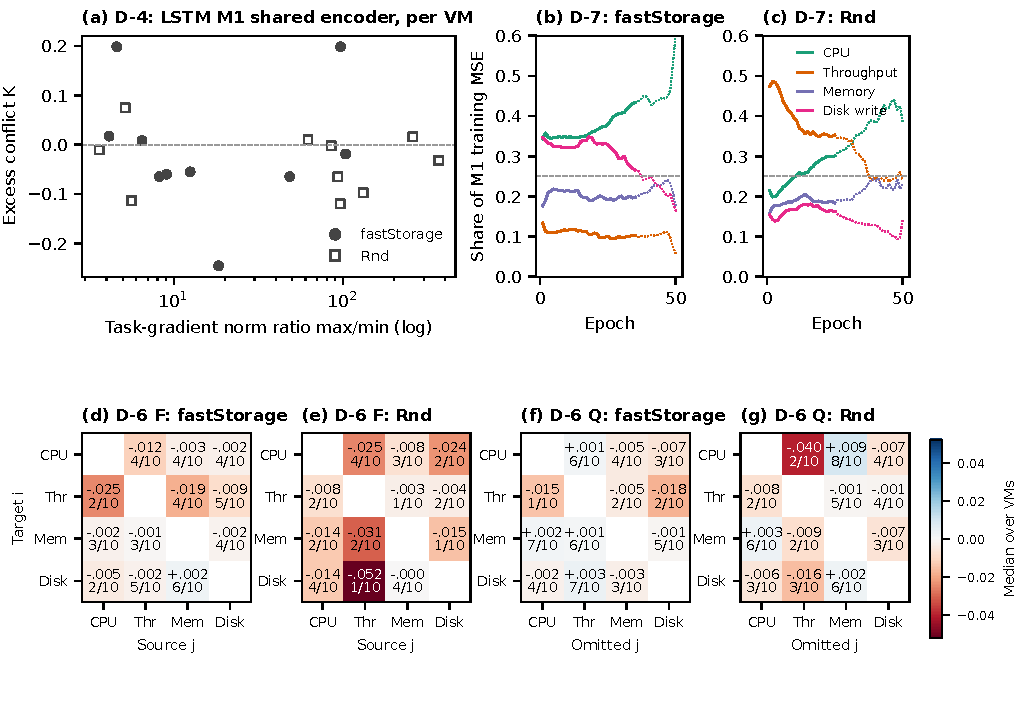
\includegraphics[width=\textwidth]{Figure_4.pdf}
\caption{Tier-2 mechanism diagnostics for the LSTM. (a) D-4 per VM: excess
sign-conflict rate $K$ against the max/min task-gradient norm ratio in the
M1 shared encoder at the selected epoch. (b)--(c) D-7: mean share of the M1
training loss by resource and epoch; solid lines cover epochs reached by at
least half of the 150 fits per resource and block, dotted lines the later
epochs reached by fewer fits; the dashed line is an equal share. (d)--(g)
D-6: median over VMs of directed transfer $F_i(j)$ and leave-one-out
contribution $Q_{i,j}$ in log-MacroMAE units (positive favours adding or
retaining $j$), with the number of VMs with a positive value. Descriptive
associations only.}
\label{fig:tier2-mechanism}
\end{figure*}

\subsection{RQ5 Resource, Environment, and Temporal Heterogeneity}
\label{sec:results-rq4}
\label{sec:cross-dataset-synthesis}

Effects varied with the resource, the environment and the temporal block, at
every prespecified level (Figure~\ref{fig:primary-gains}; Supplementary
Section~S-G). For S2:S1, CPU, throughput and disk write
change direction across evidence blocks, whereas memory is positive in five
and nearly zero and negative only in Materna T1. For sharing, fastStorage CPU
was near zero while the other three resources were negative, Rnd was broadly
negative for all four, and Materna M1-versus-S2 CPU changed from positive in
T1 to negative in T2--T3. The prespecified tier-1 criterion (RQ4 of the tier-1 protocol) for temporal
heterogeneity was met: seven of the 12 resource--comparison pairs changed
prespecified classification across T1--T3 and five changed raw sign. This is a
descriptive criterion, not an inferential claim (Supplementary
Section~S-C4).

Supplementary Table~S20 retains the prespecified TimeTrack,
equal-environment Bitbrains and equal-temporal-block Materna summaries without
a global score, with the tier-2 counts in a separate row. External memory has
favourable LSTM/Ridge contextual agreement, whereas throughput reverses
direction between families, and Materna's consecutive blocks share VM
identifiers, so their agreement is not independent replication.


\subsection{Persistence Boundary}
\label{sec:results-persistence}

Relative formulation gains do not establish superiority to a persistence
forecast. In TimeTrack, S1, S2 and M1 had positive mean skill for CPU,
throughput and disk write, but memory was the boundary ($-0.1272$, $-0.1494$
and $-0.6047$), so the large M1-versus-S2 memory penalty coincided with weak
absolute performance. Overall CPU skill was negative for S1, S2 and M1 in both
Bitbrains environments, and neither environment contained a formulation that
beat persistence for every resource. In Materna, S2 beat persistence in all 12
trace--resource overall aggregates, whereas M1 failed the check for T1 and T3
throughput and disk write.
The tier-2 backbones share this Bitbrains boundary
(Table~\ref{tab:tier2-baseline}B): on the 20-VM cohort, CPU and throughput
skill was negative for every backbone and cell, and memory and disk-write
skill positive.

\subsection{Accuracy-Efficiency Trade-Off}
\label{sec:results-efficiency}

Consolidation saves models and parameters, at the accuracy cost reported
above. The tier-1 H64 M1 consolidates the target-model complement for one entity,
outer fold and seed: one joint network and
52,500 parameters against four networks and 206,100 parameters for S2,
approximately $74.5\%$ fewer parameters and $75\%$ fewer models. The
Materna totals are 85.6 worker fit-hours for S1, 75.3 for S2 and
20.4 for M1; they are not elapsed wall time, energy or deployment cost,
and the post-hoc H129 comparison does not inherit H64's parameter-reduction
claim. In tier~2, shared LSTM, PatchTST-style and iTransformer-style models
used roughly a quarter of their independent complements' parameters, whereas
DLinear M1 was not smaller than DLinear S2 at contexts 4 and 9
(Section~\ref{sec:results-rq2}). These local inventories coexist with the
accuracy penalties above and establish no production savings.


\subsection{RQ6 Deciding Consolidation from Validation}
\label{sec:results-a3}

The sharing cost was already visible in the inner-validation errors, so a
validation check would have prevented most of it but also most of the
consolidation. Table~\ref{tab:a3} summarises A3; Supplementary Section~S-H
has every cell.

\emph{Ranking.} The shared model's validation error exceeded S2's in
\AiiiValWorseMin--\AiiiValWorseMax\% of machine--fold--seed units, more often
than its outer-test error did (\AiiiOutWorseMin--\AiiiOutWorseMax\%).
Validation and outer M1/S2 ratios were rank-correlated in \AiiiDetects{} of
\AiiiFrames{} settings (tier-1 blocks and tier-2 backbone $\times$ block;
$\rho=\AiiiRhoMin$ to $\AiiiRhoMax$), the exceptions being
\AiiiNotDetected{}, whose intervals reached zero. Validation thus ranks units
by their sharing cost, but its sign alone was near chance (balanced accuracy
\AiiiBAMin{} to \AiiiBAMax{}), because almost every unit looked worse.

\emph{Gate.} At $\tau=1\%$, G-share consolidated \AiiiRetainedOne\% of the
\AiiiUnitsOne{} tier-1 units and \AiiiRetainedTwo\% of the \AiiiUnitsTwo{}
tier-2 units, and \AiiiRetainedTwoPctOne\% and \AiiiRetainedTwoPctTwo\% at
$\tau=2\%$. Under the frozen rule this is ``rarely consolidates'' in both
tiers. Its cost cells fell from \AiiiRefCostOne{} and \AiiiRefCostTwo{} for
M1 to \AiiiCostOne{}, but this is largely mechanical: with most units kept on
S2, the median matched-cell ratio is one. A tolerance that admits sharing for
most machines would admit the cost as well.

\emph{Selective grouping.} For the tier-2 LSTM, letting validation choose
which resources share a model did better than all-or-nothing sharing. G-group
at $1\%$ used \AiiiGroupModels{} models per unit against \AiiiShareModelsLSTM{}
for G-share and 4 for S2, keeping \AiiiGroupRetained\% of the model reduction
and \AiiiGroupParamCut\% fewer parameters than S2, with no cost cell and a
largest median ratio of \AiiiGroupMaxRatio{} (M1: \AiiiMOneCostLSTM{} cost
cells, up to \AiiiMOneMaxRatio{}); the frozen verdict is ``grouping adds
savings''. Grouping did not make sharing free. Its win rates against S2 were
\AiiiGroupWinMin--\AiiiGroupWinMax\%, and \AiiiGroupMacroBelow{} of its 8
MacroMAE-gain intervals lay below zero (M1: \AiiiMOneMacroBelow{}), the
largest at $\AiiiGroupWorstGain\%$ against $\AiiiMOneWorstGain\%$ for M1. Even
the outer-test oracle needed \AiiiOracleModels{} models per unit, and only
\AiiiFixedNoCost{} of the \AiiiFixedShared{} fixed groupings that share a model
had no cost cell (Supplementary Table~S24).

\emph{Persistence fallback.} Sending a target to persistence when
persistence validated better gave positive persistence skill in
\AiiiFallbackPositive{} of the \AiiiFallbackCells{} tier-2 CPU and throughput
cells (\AiiiFallbackBefore{} without it): the persistence boundary of
Section~\ref{sec:results-persistence} is not a validation artefact.

% Generated by manuscript/fgcs/tools/a3_numbers.py; do not edit by hand.
\begin{table}[t]
\centering
\caption{Amendment A3 on existing fits. (A) Consolidation gate G-share: share of machine $\times$ fold $\times$ seed units consolidated into one shared model at tolerance $\tau$, typical-cell cost cells (policy:S2 median ratio above 1.01) and validation--test detection. (B) Tier-2 LSTM groupings at $\tau=1\%$ and $2\%$: mean models and parameters per unit, cost cells and largest median ratio (of 8 cells), and cells whose MacroMAE-gain interval lies below zero. The oracle uses the outer test and is an upper bound, not a policy.}
\label{tab:a3}
\footnotesize
\setlength{\tabcolsep}{3pt}
\begin{tabular}{@{}lccccc@{}}
\toprule
\multicolumn{6}{@{}l}{\emph{(A) G-share: units consolidated (\%), cost cells, detection}} \\
 & $\tau{=}0$ & $1\%$ & $2\%$ & Cost$_{1\%}$ (M1) & Detects \\
\midrule
Tier 1, LSTM & 4 & 8 & 14 & 0 (22) & 5/6 \\
Tier 2, 4 backbones & 7 & 20 & 29 & 0 (13) & 7/8 \\
\midrule
\multicolumn{6}{@{}l}{\emph{(B) Tier-2 LSTM, against S2}} \\
Policy & Models & Parameters & Cost & Max ratio & Macro${<}0$ \\
\midrule
S2 (independent) & 4.0 & 206{,}100 & 0 & 1.000 & 0 \\
M1 (one shared) & 1.0 & 52{,}500 & 6 & 1.057 & 5 \\
G-share, $\tau{=}1\%$ & 3.7 & 190{,}228 & 0 & 1.000 & 0 \\
G-group, $\tau{=}1\%$ & 2.4 & 124{,}180 & 0 & 1.004 & 3 \\
G-group, $\tau{=}2\%$ & 2.1 & 108{,}137 & 1 & 1.011 & 3 \\
Oracle grouping & 2.8 & 144{,}489 & 0 & 1.000 & 0 \\
\bottomrule
\end{tabular}
\end{table}


\section{Discussion}
\label{sec:discussion}

\subsection{When Cross-Resource Context Helps}
\label{sec:discussion-context}

Cross-resource context is worth adding only for some resources and models.
Cross-family agreement for external memory, TimeTrack's reversal and T1's
seed-variable estimate support selective contextual value, not a universal
memory benefit, in line with MMRP's non-uniform contextual gains
\citep{Tripathi2025MMRP} and the relevance of environment-specific evaluation
\citep{Rossi2025CloudUncertainty}.
Tier~2 extends the model-family dependence from Ridge to three further
backbones. Context effects were small, and their direction depended on the
backbone: memory improved for the LSTM and DLinear but not for PatchTST, and
no context cell held across backbones. For the PatchTST-style backbone, adding
the other resources made forecasts worse: in 4 of its 8 S2:S1 cells the
median-ratio interval lay wholly above one under VM resampling, against none
for the LSTM (Supplementary Table~S19). This matches the robustness that
\citet{Han2024ChannelIndependent} report for channel-independent models.
Contextual value is therefore a
property of a resource, an environment and a model family together, not of
the telemetry alone.

\subsection{Shared Representation and Adverse Transfer}
\label{sec:discussion-sharing}

For a typical machine, sharing cost accuracy in almost every comparison. The
sensitivity controls retain adverse throughput, memory and disk-write points
across all six blocks, and direction need not imply uniform severity: Materna
T1/T3 disk-write median ratios are about $1.025/1.035$,
despite much larger tail-sensitive MacroMAE penalties.

The adverse direction is not specific to the LSTM, although its size
largely is: in tier~2, all-input sharing lowered MacroMAE accuracy in 29 of
32 cells, but its magnitude, class and interaction with input scope depended
on the backbone, and only two cells, both own-input sharing on Rnd, met the
strict cross-backbone rule. DLinear M0 is the most extreme
form of sharing evaluated, one linear map tied across all four resources
without resource-specific outputs, and its Rnd CPU penalty is dominated by a
single high-scale VM (Section~\ref{sec:results-rq2}).

Useful task-dependent transfer is established
\citep{Caruana1997Multitask,Standley2020TaskGrouping,Fifty2021TaskGroupings},
including in forecasting \citep{Nikentari2022NARMAXLSTM,Nochumsohn2025MTLinear},
so the question is which explanation fits here. For the LSTM
(Section~\ref{sec:results-diagnostics}), near-orthogonal task gradients rule
out the destructive conflict that gradient surgery targets
\citep{Yu2020GradientSurgery}, whereas strongly unequal gradient magnitudes
and loss shares fit one task's loss dominating the shared parameters despite
equal nominal weights (Section~\ref{sec:m1}), the imbalance that
loss-balancing methods address \citep{Chen2018GradNorm}. Dependence and
pairwise transfer were not consistently associated with the effects.

Amendment A1 tested the imbalance account directly. Uncertainty weighting
reduced the effective imbalance and improved the shared LSTM in every cell,
but by at most 0.4\% in median matched-cell error, and the shared model
stayed less accurate than S2. For this model, loss balancing is therefore a
partial remedy, not a removal of the sharing cost. A3 then tested the
task-grouping response \citep{Standley2020TaskGrouping,Fifty2021TaskGroupings}:
sharing only the resources that validation admits kept about half of the
LSTM's model reduction at a typical-cell cost below 0.5\%, but not the
aggregate accuracy of S2. Which resources a machine shares, rather than
whether it shares, carried most of the remaining savings; gradient-aware and
multi-objective designs \citep{Sener2018MultiObjective,Yu2020GradientSurgery}
remain untested.

\subsection{Implications and the Accuracy-Consolidation Trade-Off}
\label{sec:discussion-systems}
\label{sec:discussion-efficiency}

Forecasting supports adaptation
\citep{Taherizadeh2018Monitoring,Bauer2020SelfAware}. The inner-validation
errors computed during model selection ranked machines by their sharing cost
before any
test data were seen, so a forecasting service can gate consolidation per
machine at no extra training cost. A strict gate mostly declines to share; a
grouping gate keeps about half of the model reduction at a small typical-cell
cost, an explicit accuracy--compactness trade-off
\citep{Standley2020TaskGrouping,Syu2017DynamicQoS}. Adverse aggregate tails
remained under grouping and still need checking.

\subsection{Applicability and Generalisation Limits}
\label{sec:discussion-applicability}

Applicability is bounded by the limits in Section~\ref{sec:threats}, and
cross-family reversals do not select a universal replacement. The tier-2
backbones show that the sharing direction recurs beyond the LSTM, not how
tuned modern architectures would rank, and adaptive or hybrid sharing remains
untested \citep{Yu2020GradientSurgery,Nochumsohn2025MTLinear}.
Global models remain outside this evaluation
\citep{MonteroManso2021GlobalForecasting}.
The same limit applies to foundation forecasters
\citep{DiMenna2026RuntimeForecasting}. Future comparisons should retain
independent all-input controls and resource-specific assessment, and test
loss balancing beyond the LSTM, which is the only backbone A1 covered.

\subsection{What the Separation Means in Practice}
\label{sec:discussion-separability}

The two decisions behaved differently, which changes how they should be
tested. Context effects were small and their direction depended on the
resource, the environment and the backbone, so a contextual input should be
adopted only after a per-resource, per-model check. Sharing had a
typical-cell cost whose direction held across backbones, so consolidation
should be justified by its savings and checked for adverse tails rather than
assumed free; A3 shows that inner validation can make that check. The two can
disagree for the same target:
context helped LSTM Rnd memory while sharing still cost accuracy, and in Rnd
the sharing cost appeared with own-resource input as well. A contextual
benefit is not a reason to consolidate, and a consolidation saving is not
evidence that
cross-resource information is being used.

\section{Threats to Validity}
\label{sec:threats}

\subsection{Construct Validity}
\label{sec:threats-construct}

Tier~1 has three of the four $2\times2$ cells; M0 exists only in tier~2, on a
reduced cohort, and tier-2 cells are defined by backbone structure:
iTransformer S1 and M0 are undefined, DLinear M0 ties one map across all four
resources without resource-specific outputs, and DLinear M1's width-16
bottleneck has lower rank than four S2 maps at context 4, so DLinear M1:S2
partly reflects reduced capacity. The transformer-style backbones are declared
adaptations, and resource mappings are source-specific rather than perfectly
equivalent. MacroMAE gains describe one error estimand; metric choice can
alter rankings \citep{Hyndman2006Accuracy}, and scaled-space training differs
from native-unit evaluation. Results are reported per resource over all
horizons: horizons enter only through the classes' horizon-consistency
thresholds and the pooled matched cells, and no horizon-specific claim is
made. The study evaluates established backbones and losses rather than
proposing a new architecture, and its diagnostics describe associations, not
a unique sharing mechanism. It measures forecast accuracy and model
consolidation, not autoscaler, scheduler or SLA outcomes: forecast error is
what the consolidation decision changes directly, whereas controller outcomes
also depend on policy and platform \citep{Qu2018Autoscaling}.

\subsection{Internal Validity}
\label{sec:threats-internal}

The mechanisms of Section~\ref{sec:validation-strategy} constrain leakage and
implementation error \citep{Cerqueira2020Evaluation,Hyndman2021Forecasting}
but cannot exclude every implementation or data error. The tier-1 sensitivity
controls are post hoc and address context and capacity separately, not
jointly. Only three neural seeds were recorded: 9/24 S2:S1 and 4/24 M1:S2
tier-1 block/resource summaries change sign across them (Supplementary
Table~S2). Tier~2 fixes hyperparameters and uses the LSTM-selected H64-M1
context for every backbone. This keeps each contrast within one fixed model
and prevents tuning effort from differing between cells, but the modern
backbones may be under-tuned and their absolute ranking is not established;
the largest tier-2 aggregate was stable across seeds, with per-VM seed spreads
outside VMs 233 and 269 of at most 0.046 native units. Gradient diagnostics
cover only the LSTM at the selected epoch, D-2 reuses Ridge outcomes already
observed, and Ridge uses a finite five-alpha grid at LSTM-selected contexts.

\subsection{External Validity}
\label{sec:threats-external}

The sources represent particular runtime and cloud contexts, not probability
samples of all VMs, and Materna's blocks are repeated-within-source evidence.
Tier~2 covers 20 of the 70 Bitbrains VMs from one trace family, with no
Materna or TimeTrack data; tier~1 remains the full-cohort evidence. Canonical
or tuned transformer forecasters, mixture-of-experts, adaptive sharing,
gradient surgery and foundation forecasters were not tested, loss balancing
and selective grouping were tested for the LSTM only, and four resource
semantics do not establish accuracy for application latency or QoS.

\subsection{Conclusion Validity}
\label{sec:threats-conclusion}

Because native errors are not rescaled across entities, one high-scale VM
can set an aggregate: VM233 contributes $98.6\%$ of the DLinear Rnd CPU
M0$-$S1 excess behind its $-139.61\%$ gain, so tier-2 magnitudes are read
together with matched-cell medians, win rates and per-VM counts. For
Bitbrains CPU and throughput, the contrasts compare forecasters that are all
less accurate than persistence (Section~\ref{sec:results-persistence}), so
the sharing and context effects there describe relative behaviour among such
forecasters, not usable accuracy; the limit does not apply where skill was
positive, as for tier-2 memory and disk write and every Materna S2 aggregate.

The VM-cluster intervals resample machines over seed-averaged errors, so they
exclude seed variation, which is reported separately as sign changes. With
ten VMs per block, tier-2 percentile intervals are wide and may under-cover:
they indicate direction rather than precise size, and tier~2 makes no
confirmatory claim. Intervals exist for the tier-1 MacroMAE gains and the
tier-2 median ratios but not for the tier-1 median ratios, and TimeTrack has
none. Counts of intervals that exclude one or zero are not family-wise
corrected, so some exclusions are expected by chance. The intervals condition
on the evaluated cohorts; overlapping folds, multiple horizons, repeated seeds
and dependent Materna blocks are not IID replicates, and no global effect or
meta-analysis is used.

The tier-2 diagnostics are associations across at most ten VMs per block
and two environments; the coincidence of larger gradient imbalance and
broader sharing penalties in Rnd is one comparison of two blocks, not an
estimated relationship. Amendment A1 was motivated by those diagnostics, so
its hypothesis was chosen after they were seen, although it was frozen before
any A1 fit; it covers one backbone, 20 VMs, three seeds and fixed balancing
settings. Amendment A3 was likewise specified after the component
models' outer errors were known, although none of its policy outcomes had
been computed when it was frozen. Its typical-cell cost counts are
insensitive when a policy keeps most units on S2, so its savings and MacroMAE
intervals carry the comparison, and its gates compare scaled validation MAE
(tier~1) or MSE (tier~2) with native outer MAE (full threats: Supplementary
Section~S-D).

\section{Conclusion}
\label{sec:conclusion}

Varying contextual input and representation sharing one at a time, under
frozen protocols and the checks of Section~\ref{sec:validation-strategy},
shows that their consequences differ. Representation sharing carried a
recurring accuracy cost: for a typical machine, the shared model was less
accurate in all 24 tier-1 LSTM comparisons and in 30 of 32 tier-2 backbone,
resource and environment cells. The cost exceeded $1\%$ in 6 of 8 tier-2 LSTM
cells but in only 7 of 24 cells of the other backbones, and the tier-1
throughput, memory and disk-write penalties remained in all six blocks under
the common-context and approximately capacity-matched controls. Aggregate
MacroMAE penalties were larger and less uniform, because a few high-scale
machines dominate native-unit errors. Contextual input gave small and
selective benefits, most consistently for memory in the external
environments, and no tier-2 context effect held across backbones.

In the shared LSTM, task gradients were near orthogonal, not in conflict, but
strongly unequal in magnitude and loss share; balancing the losses made the
shared LSTM slightly more accurate in every cell, but not as accurate as the
independent all-input models. The cost is visible before deployment:
inner-validation errors ranked machines by their sharing cost in
\AiiiDetects{} of \AiiiFrames{} settings, so a gate sharing only within 1\%
consolidated \AiiiRetainedOne--\AiiiRetainedTwo\% of units, whereas
validation-chosen grouping kept \AiiiGroupRetained\% of the LSTM's model
reduction at typical-cell ratios of at most \AiiiGroupMaxRatio{}, although
some aggregate costs remained. For multi-metric telemetry, the practical
question is therefore which resources to share rather than whether to share,
and the validation data needed to answer it already exist. These conclusions
hold for typical machines on the evaluated cohorts; on the 20 Bitbrains VMs no
backbone beat persistence for CPU or throughput, and a validated fallback made
only \AiiiFallbackPositive{} of \AiiiFallbackCells{} such cells positive.

\section*{Data availability}

TimeTrack is publicly available on
\href{https://www.kaggle.com/datasets/abdelghanimeliani/open-air-interface-cicd-timeseries-dataset}{Kaggle}
(Apache 2.0 in its dataset metadata) and in the publisher's
\href{https://doi.org/10.5281/zenodo.15442251}{Zenodo archive
(doi:10.5281/zenodo.15442251; CC BY 4.0)}; its description paper is
\citet{Meliani2025TimeTrack}. Bitbrains fastStorage and Rnd are publicly
available as \href{https://atlarge-research.com/gwa-t-12/}{GWA-T-12}
\citep{Shen2015Bitbrains}, and Materna T1--T3 as
\href{https://atlarge-research.com/gwa-t-13/}{GWA-T-13}
\citep{Kohne2014FederatedCloudSim,Kohne2016SLAScheduling}. We acknowledge
Bitbrains IT Services Inc. and Materna GmbH Information \& Communications for
providing these traces through the Grid Workloads Archive; their source pages
specify acknowledgement and citation conditions rather than a standard
open-data licence, and readers should obtain the raw data from these sources.

All code is in the public repository \url{https://github.com/KADOUMAAbdelhak/TimeTrack-Forecasting-Framework}.
Source code, protocols, derived analysis outputs and SHA-256 inventories for
the tier-1 experiments, post-hoc controls and robustness diagnostics are at
the
\href{https://github.com/KADOUMAAbdelhak/TimeTrack-Forecasting-Framework/tree/0e8cad884896a706f62f0fae4ab2b52812f9b033}{project repository checkpoint}
\texttt{\seqsplit{0e8cad884896a706f62f0fae4ab2b52812f9b033}}; fitted-model and
per-fit prediction collections are identified by checksum inventories but not
included. The tier-2 protocol, code, configuration, input digests, execution
seal and launcher are frozen by the annotated tag
\href{https://github.com/KADOUMAAbdelhak/TimeTrack-Forecasting-Framework/tree/fgcs-v04-min-final-r2}{\texttt{fgcs-v04-min-final-r2}}
(commit \texttt{\seqsplit{7ef468c0cc21c1c8ca33bfd9db0ee919e0dee24a}}; the suffix
``r2'' marks a second tag of the same frozen package, created before any tier-2
run, not a manuscript revision), and sealed inputs not held in Git are archived on Zenodo
(\href{https://doi.org/10.5281/zenodo.24189108}{doi:\allowbreak 10.5281/\allowbreak zenodo.24189108}).
The tier-2 analysis output (SHA-256
\texttt{\seqsplit{308841865ec87b04e10ecb64f20bc13ce2e671511a1574056028f7b5710dd17a}})
and the DLinear Rnd CPU audit summary (SHA-256
\texttt{\seqsplit{88b6f56a81d2db8eb87a4d878569c95595c247f1368dd2c8460429dbbb9a1b58}}),
with the closed tier-2 journal records and a file-level SHA-256 inventory, are
archived on Zenodo
(\href{https://doi.org/10.5281/zenodo.24339239}{doi:\allowbreak 10.5281/\allowbreak zenodo.24339239},
version v0.4-outputs; launcher records with local paths redacted, model
weights not included), and the tier-2 figures and tables are generated by
scripts that verify these digests. Amendment A1 (protocol, code,
configuration, package and execution seal) is frozen by the annotated tag
\href{https://github.com/KADOUMAAbdelhak/TimeTrack-Forecasting-Framework/tree/fgcs-v04-a1-intervention}{\texttt{fgcs-v04-a1-intervention}}
(commit \texttt{\seqsplit{7660bde98cb4f47d51226877b8f8c8235d1b9201}}). Its
analysis output (SHA-256
\texttt{\seqsplit{ad0c4151dc9283c90336794f82bc3b5e7e2b9d90e92d52b416c55c6c7d720062}})
and closed journal records are archived on Zenodo
(\href{https://doi.org/10.5281/zenodo.24353235}{doi:\allowbreak 10.5281/\allowbreak zenodo.24353235};
launcher records with local paths redacted, model weights not included).
Amendment A3 (protocol, configuration, code and tests) is frozen by the
annotated tag
\href{https://github.com/KADOUMAAbdelhak/TimeTrack-Forecasting-Framework/tree/fgcs-v04-a3-validation-gate-r2}{\texttt{fgcs-v04-a3-validation-gate-r2}}
(commit \texttt{\seqsplit{9ca21ff7c4823406bc0f82ffdbbd567e36a631a4}}; ``r2'' re-tags, without
internal notes, the byte-identical package tagged before the A3 run). Its
output (SHA-256
\texttt{\seqsplit{33e11a858ea338b3c3ff25bec2f59527a3a2100a386658443def77956501cee0}})
and run record are in the repository and, with the tier-1 inputs it read,
on Zenodo
(\href{https://doi.org/10.5281/zenodo.24458960}{doi:\allowbreak 10.5281/\allowbreak zenodo.24458960}).
Amendment A2 (change-from-last-value forecasting), frozen under tag
\texttt{fgcs-v04-a2-residual}, has not been executed; no A2 result is reported.
An OSF registration (\href{https://osf.io/kuwra}{kuwra}) of a superseded
tier-2 protocol draft is retained.

\section*{CRediT authorship contribution statement}

\textbf{Abdelhak Kadouma:} Conceptualization, Methodology, Software, Data curation, Formal analysis, Validation, Visualization, Writing -- original draft. \textbf{Amit K. Shukla:} Supervision, Conceptualization, Methodology, Writing -- review \& editing. \textbf{Mohammed Elmusrati:} Supervision, Project administration, Writing -- review \& editing.


\section*{Funding}

This research did not receive any specific grant from funding agencies in
the public, commercial, or not-for-profit sectors.

\section*{Declaration of Competing Interest}

The authors declare that they have no known competing financial interests or
personal relationships that could have appeared to influence the work reported
in this paper.

\section*{Declaration of generative AI and AI-assisted technologies in the manuscript preparation process}

During the preparation of this work, the authors used OpenAI ChatGPT and Codex
to assist with drafting and revising selected manuscript text, language editing
and proofreading, and the development and review of portions of the code used
for post-hoc analyses and reproducibility checks. For tier~2 and
its amendments, the authors also used Anthropic Claude (Claude Code) to assist
with developing and reviewing tier-2, analysis, audit and
figure-generation code, and with drafting and revising manuscript and
supplementary text. After using these tools, the
authors reviewed, edited, and validated the outputs as needed and take full
responsibility for the content, accuracy, integrity, and originality of the
published article. Figures and tables were rendered by deterministic code
from the frozen results; no figures, images, or visual elements were
generated directly by generative AI tools.


\bibliographystyle{elsarticle-num-names}
\bibliography{references}

\end{document}
